%-----------------------------------------------------------------------
% PHYSICS HONOURS THESIS
% AUTHOR    : MICHAEL PAPASIMEON
% DATE      : NOVEMBER 1998
%-----------------------------------------------------------------------

\documentclass[a4paper,titlepage]{sfreport}
%\documentclass[a4paper,titlepage,aps]{revtex}

%-----------------------------------------------------------------------
% LATEX PACKAGES
%-----------------------------------------------------------------------
\usepackage{helvet}
\usepackage{a4wide}
\usepackage{amsmath}
\usepackage{amsxtra}
\usepackage{fancybox}
%\usepackage{fancyheadings}
\usepackage{fancyhdr} 
\usepackage{multicol}
\usepackage{float}
\usepackage{tabularx}
\usepackage{graphicx}
\usepackage{layout}
%\usepackage{pslatex}

%----------------------------------------------------------------------
% PAGESTYLE
%----------------------------------------------------------------------

\pagestyle{fancyplain}
%\setlength{\voffset}{0pt}
%\setlength{\topmargin}{0pt}
%\setlength{\textheight}{670pt}
%\setlength{\marginparwidth}{0pt}

%----------------------------------------------------------------------
% LATEX MACROS
%----------------------------------------------------------------------
\restylefloat{table}

\newcommand{\mb}[1]{\mathbf{#1}}
\newcommand{\ket}[1]{|#1 \rangle}
\newcommand{\bra}[1]{\langle #1|}
\newcommand{\Alpha}{\bar{\alpha}}
\newcommand{\Exp}[2]{e^{i \mb{#1} \cdot \mb{#2} }}
\newcommand{\ExpM}[2]{e^{-i \mb{#1} \cdot \mb{#2} }}
\newcommand{\state}[2]{\psi_{#1 #2}}
\newcommand{\Muq}{\mu(\mb{q},\theta,\phi)}
\newcommand{\Angstrom}{\stackrel{\circ}{\mathrm{A}} }
\newcommand{\InvAngstrom}{ \stackrel{\circ}{\mathrm{A}}^{-1} } 
\newcommand{\Half}{\frac{1}{2}}

\setcounter{tocdepth}{10}
\setcounter{secnumdepth}{10}

\setlength{\parindent}{0pt}
\setlength{\parskip}{1.3ex}

%\renewcommand{\chaptername}{Part}
\renewcommand{\contentsname}{Contents}
\renewcommand{\bibname}{References}

\newcommand{\HRule}{\rule{\textwidth}{1mm}}
\newcommand{\Trule}{\rule{\textwidth}{0.1pt}}

\newcommand{\maketitlepage}[2]{
    \begin{titlepage}
    \vspace*{\stretch{1}}
    \HRule
%    \begin{flushright}
\begin{center}
        {\textsf{{ \huge  #1} }}
        \\[5mm]
        \Trule
        \\[5mm]
        \Large \textsf{#2}
\end{center}
%    \end{flushright}
    \HRule
    \vspace*{\stretch{2}}
    \begin{center}
        
\includegraphics[height=4cm]{UMCrest97.eps}
    \end{center}
    \begin{center}
        \Large\textsc{1998 Physics Honours Thesis \\
                      Optics Group, School of Physics\\
                      The University of Melbourne \\
                      November 16, 1998}
    \end{center}
    \end{titlepage}
}

\newcommand{\Section}[1]{\subsection{#1}}
\newcommand{\Subsection}[1]{\subsubsection{#1}}
\newcommand{\Subsubsection}[1]{\paragraph{#1}}

\newenvironment{Boxedminipage}%
    {\begin{Sbox}\begin{minipage}}%
    {\end{minipage}\end{Sbox}\fbox{\TheSbox}}
\newcommand{\Startbox}[1]{\begin{Boxedminipage}{\textwidth}%
            {\large \sffamily{#1}} \vspace{1mm} \hrule \vspace{2mm} }
\newcommand{\Endbox}{\end{Boxedminipage}}

\newcommand{\bt}{\begin{center}\begin{tabular}%
                {|>{\sffamily}m{6cm}|>{\sffamily}m{2cm}%
                 |>{\sffamily}m{2cm}|>{\sffamily}m{2cm}|} \hline %
                \bfseries{Requirement} & \bfseries{TCSEC} & %
                \bfseries{ITSEC} & \bfseries{CTCPEC} \\ \hline \hline}
\newcommand{\et}{\end{tabular}\end{center}}
\newcommand{\cmp}[4]{#1 & #2 & #3 & #4 \\ \hline}

%----------------------------------------------------------------------
% COMMANDS TO CONSTRUCT FANCY HEADINGS
%----------------------------------------------------------------------

%\addtolength{\textwidth}{\marginparsep}
%\addtolength{\textwidth}{\marginparwidth}

%\addtolength{\headwidth}{\marginparsep}
%\addtolength{\headwidth}{\marginparwidth}

%\setlength{\footrulewidth}{0.4pt}
%\setlength{\plainfootrulewidth}{0.4pt}

\renewcommand{\headrulewidth}{0.4pt}
\renewcommand{\plainheadrulewidth}{0.4pt}
\setlength{\parindent}{0pt}
\setlength{\parskip}{1.3ex}

\renewcommand{\chaptermark}[1]{\markboth{#1}{}}
\renewcommand{\sectionmark}[1]{\markright{\thesection\ #1}}

\lhead[\fancyplain{\small\it\thepage}{\small\it\thepage}]%
      {\fancyplain{\small\it\rightmark}{\small\it\rightmark}}
\rhead[\fancyplain{\small\it\leftmark}{\small\it\leftmark}]%
      {\fancyplain{\small\it\thepage}{\small\it\thepage}}
\cfoot{}

%----------------------------------------------------------------------
% MAIN DOCUMENT
%----------------------------------------------------------------------

\begin{document}
    \pagenumbering{roman}
    \maketitlepage{Investigation of Theoretical Approaches for\\
                   \vspace{3mm} 
                   Computing Relativistic Atomic Form Factors}%
                   {Author: Michael Papasimeon 
                   \\[5mm]
                   Supervisor: Dr. Christopher T. Chantler} 

    \chapter*{Abstract}
    The calculation of accurate atomic form factors is of great importance in
    fields such as crystallography and medicine, as they provide valuable 
    information about how photons (especially in the X-ray regime)
    interact with matter.
    Theoretical methods for calculating relativistic atomic form factors 
    are investigated with an emphasis on the Hydrogen atom.
    New results and comparisons with other theories for relativistic normal form 
    factors for hydrogenic atoms are presented.
    Anomalous form factor calculations using a relativistic S-matrix approach
    are also computed for hydrogen using an ``all-poles'' and the electric
    dipole approximation.
    \vspace*{10cm}
    \hrule
    \vspace*{5mm}
    I authorize the Chairman of the School of Physics to make or have made a
    copy of this report for supply to any person judged to have an
    acceptable reason for access to the information, i.e., for research,
    study or instruction.
    \vspace*{10mm}
    \begin{flushright}
    Signature.....................................
    \end{flushright}
    \vspace*{5mm}
    \hrule

    \chapter*{Acknowledgements}
    I would like to offer my greatest gratitude and thanks to my supervisor 
    Dr. Chris Chantler, for his guidance, time, effort, suggestions, ideas, corrections,
    for his great enthusiasm for atomic physics and for being a great guy.
    He is the person responsible for focusing my attention as a third year
    student onto atomic physics and therefore gave me the opportunity
    to have an additional fascinating perspective into the physical world.

    I would also like to thank my fellow honours students, in particular
    Karen Violante, Magda Michna and Tom Hunt who I shared an office with for a
    year, and who with I had some great times (and some stressful and worrying times
    especially during exams).

    I would also like to thank the members of the Optics group, and the
    lecturers of my fourth year subjects, Geoff Opat, Lloyd Hollenberg, Ann
    Roberts, Rob Scholten, Ken Amos and Rachel Webster.

    \tableofcontents
    \listoffigures

    % CHAPTER 1 - INTRODUCTION
    \chapter{PROJECT OVERVIEW AND ATOMIC FORM FACTOR THEORY}
        \pagenumbering{arabic}
        
\section{Introduction}
The use of high energy radiation has many wide spread uses. In particular,
the understanding of how radiation in the X ray regime interacts with matter 
has applications in areas such as astronomy, medicine and in the study of the
structure of materials such as in the field of crystallography.

In order to be able to interpret results of experiments which make use of X rays
or other high energy photons we must understand how such photons interact with
matter. The most fundamental process that can be considered is the interaction
of a single photon with a single isolated atom. This can include the study of
coherent and incoherent scattering processes, photoionisation, photoabsorption
and pair production.

In particular, the theoretical calculation of atomic form factors allows the
determination of quantities such as cross sections and attenuation coefficients
which are valuable in obtaining information about the atom-photon interaction
process.

The study of atom-photon interactions through the calculation of atomic form
factors covering all elements has been the subject of decades of experimental
and theoretical research. This work includes the synthesis by Henke~\cite{Henke-Experimental}
of experimental and theoretical results, theoretical results using the
relativistic dipole approximation of Cromer and
Libermann~\cite{Cromer-1,Cromer-2,Cromer-3}, theoretical results of Kane et al.
based on S-matrix theory~\cite{Kane-Kissel-Pratt}, recent theoretical
tabulations by Chantler~\cite{Chantler-Tabulation}, the results of
Saloman, Hubbell and Scofield~\cite{Saloman-Hubbell-Scofield} and the results
of Creagh~\cite{Creagh-Hubbell,Creagh-McAuley}.

\section{Project Aims}
Major improvements on current results~\cite{Chantler-Book}
would also involve many years of additional research.
However, a detailed comprehension of the assumptions made in research to date 
may be made by a detailed and critical study of form factor calculations for
hydrogen; in particular looking at the different assumptions and methods used to
compute atomic form factors.
This study of hydrogen allows us to show new results for:
\begin{enumerate}
    \item Analytic forms for the relativistic normal form factor for hydrogenic 
          atoms.
    \item Numerical results for imaginary
          component of the anomalous form factor for hydrogen using a
          relativistic S-matrix approach.
    \item The angular dependence of the photionisation differential cross
          sections at selected energies.
    \item Semi-analytic results for hydrogenic bound-bound transition matrix elements.
\end{enumerate}


        
\section{Atomic Form Factor Theory}
The atomic form factor is given by the x-ray scattering amplitude $f$ 
which by convention separated into a number of components. 
It is commonly written as~\cite{Chantler-Book}
\begin{equation}
    f = f_0 + f' + if''
\end{equation}
where $f_0 = f_0(q,Z)$ is known as the normal or coherent scattering amplitude
and is a function of momentum transfer $q$ and atomic number $Z$.
The anomalous scattering component (also known as the anomalous dispersion or
resonant scattering component) has real and imaginary parts given by $f'$ and
$f''$. The anomalous component is a function of the incident photon energy.
In the literature $f'$ and $f''$ are also known as $f_1$ and $f_2$.

\subsection{Normal Component}
The normal component of the atomic form factor is defined as the Fourier
transform of an atom's electronic charge density~\cite{Crasemann}.
The expression for $f_0(q)$ with an atom with electronic charge density
$\rho(\mb{r})$, is given below with the second equation being valid for the case
of a spherically symmetric atom~\cite{Chantler-Book}.
\begin{equation} \label{eq:nff-spherical}
    f_0(q) = \int \rho(\mb{r}) e^{i\mb{q}\cdot\mb{r}} \; d\mb{r}
           = \int_0^\infty \rho(r) \frac{\sin(qr)}{qr} r^2 \; dr
\end{equation}
The momentum transfer is defined as
\begin{equation}
    q = |\mb{k_{final}} - \mb{k_{initial}}| = \frac{4\pi \sin(\theta/2)}{\lambda}
\end{equation}
where $\lambda$ is the wavelength of the incident photon and $\theta$ is the
scattering angle. It is conventional to measure the momentum transfer $q$
in inverse Angstroms ($\InvAngstrom$).
  
\subsection{Anomalous Component}
The imaginary part of the anomalous form factor is related to the total
photoionisation cross section.
\begin{equation} \label{eq:fpp-sigma}
    f''(\omega) = \frac{\omega}{4\pi c r_0} \sigma(\omega)
\end{equation}
The photon energy is given by $\hbar\omega$, $c$ is the speed of light and $r_0$
is the classical electron radius. The photionisation cross section 
$\sigma(\omega)$ may also include cross sections from bound-bound
transitions.

The $f'$ component may be computed from the $f''$ component using a 
dispersion relation.
\begin{equation}
    f'(\omega) = f'(\infty) - \frac{2}{\pi} P
                 \int_0^\infty 
                 \frac{\omega' f''(\omega')}{\omega^2 - {\omega'}^2} \; d\omega'
\end{equation}

\subsection{Theoretical Limitations and Assumptions}
The theoretical calculations of atomic form factors are usually made with a
number of limitations and/or assumptions. These fall into a number of different
categories. Improvements to existing theories attempt to eliminate one or more
of these assumptions or limitations.

\begin{description}
    \item[\it 1. ATOMIC STRUCTURE :] 
    For a simple atom such as hydrogen, the quantum
    mechanical wave-functions of an atom may be either non relativistic (standard
    Schr\"odinger wave-functions), or relativistic (four component Dirac
    spinors). For many-electron atoms there is still a choice between non
    relativistic and relativistic wave-functions but additional choices have
    to be made as how to compute these wave-functions as analytic solutions
    are not available. Methods for computing many electron wave-functions include
    Hartree-Fock (HF), Dirac-Hartree-Fock (DHF), Hartree-Slater (HS), 
    Multi-Configuration-Dirac-Fock
    (MCDF) and all orders methods which include quantum electrodynamic
    corrections~\cite{Sapirstein}. Although issues such as the suitability of the
    independent particle approximation (IPA) and the computational methods used
    to determine atomic structure are important in the areas of atomic physics,
    many body perturbation theory and computational chemistry, they are also of
    relevance to form factor theory due to the reliance on accurate
    computed wave-functions.
    \item[\it 2. ELECTROMAGNETIC FIELD :]
    The incident photon is modeled as either a classical or quantised
    electromagnetic field. The simpler approach of using a classical
    electromagnetic field is more common and approximations to this model
    involve considering only the electric dipole (E1) and/or electric quadrupole
    (E2) approximations. Alternatives includes using a relativistic multipole
    (RMP) or an ``all-poles'' approach can be taken in
    which no approximations to the classical electromagnetic field are made.
    \item[\it 3. ISOLATED ATOM :]
    Most form factor calculations are done for a single isolated atom. However,
    experimentally it is extremely difficult if not impossible to obtain results
    from an isolated atom. As a result, there are inherent limitations in
    theories which consider only the case of an isolated atom. Experimentally,
    effects such as XAFS (X-ray Anomalous Fine Structure) arise from multiple
    scattering processes off multiple atoms.
    \item[\it 4. PERTURBATION THEORY :]
    Models of atom-photon interactions usually treat the electromagnetic field
    model of the photon as a small perturbation, and such there are a number of
    approaches in computing the required matrix elements and relevant scattering
    amplitudes. The main issue involves the order of the perturbation theory 
    (usually first or second order) and the type of perturbation theory used -
    standard (time dependent or time independent), relativistic perturbation
    theory and second order S-matrix theory which is obtained from covariant
    perturbation theory.
    \item[\it 5. ADDITIONAL PROCESSES :]
    A number of processes can occur when a photon interacts with an atom. 
    An atomic form factor calculation usually includes one or more of these
    processes. These processes include:
        \begin{itemize}
            \item Photoionisation
            \item Bound-Bound Transitions
            \item Rayleigh (Coherent) Scattering
            \item Compton (Incoherent) Scattering
            \item Delbr\"uck Scattering
            \item Pair Production
            \item Nuclear Thomson Scattering
        \end{itemize}
    \item[\it 6. NUMERICAL AND COMPUTATIONAL :]
    Form factor calculations require considerable computational work. Therefore
    a number of numerical computation issues need to be considered. These
    includes choices for integration and interpolation methods, numerical
    precision, convergence and computation time.
\end{description}








    % CHAPTER 2 - ATOMIC STRUCTURE
    \chapter{REVIEW OF ATOMIC STRUCTURE}
        %============================================================================
% ATOMIC STRUCTURE DEFINITIONS AND CONSTANTS
%============================================================================

This section describes the atomic structure information required for the form
factor calculations such as physical constants, definitions, atomic energy
levels and atomic wave functions.

%============================================================================
% CONSTANTS
%============================================================================
\section{Constants and Definitions}
We first need to define the usual symbols which are common in atomic physics.
\begin{center}
\begin{tabular}{|c|l|} \hline
    Symbol                  &   Meaning                     \\ \hline \hline
    $c$                     &   Speed Of Light              \\
    $e$                     &   Electron Charge             \\
    $m$                     &   Electron Mass               \\
    $a_0$                   &   Bohr Radius                 \\ 
    $\alpha$                &   Fine Structure Constant     \\
    $\hbar$                 &   Planck's Constant/$2\pi$    \\
    $r_0$                   &   Classical Electron Radius   \\
    $Z$                     &   Atomic Number               \\
    $Y_{lm}(\theta,\phi)$   &   Spherical Harmonics         \\
    \hline
\end{tabular}
\end{center}
We will use $\mb{k} = (k_x,k_y,k_z)$ to represent the photon wave propagation
vector, and in the case of photoionisation, we will use $\mb{k'} =
(k'_x,k'_y,k'_z)$ for the wave-vector of the ejected electron.
Electronic coordinates with respect to the nucleus will be denoted by 
$\mb{r} = (r,\theta,\phi)$ whereas the ejection angles of a photo-electron will
be denoted by $\Omega = (\Theta,\Phi)$.
In order to avoid confusion with the fine structure constant $\alpha$,
the Dirac alpha matrix will be denoted by $\Alpha$ where
\begin{equation}
    \Alpha = 
    \left(
        \begin{array}{cc}
            0                           &   \mbox{\boldmath $\sigma$} \\
            \mbox{\boldmath $\sigma$}   &   0
        \end{array}
    \right)
\end{equation}
and where $\mbox{\boldmath $\sigma$}$ are the Pauli spin matrices.

When dealing with four component spinors the following definitions have been
adopted.
\begin{itemize}
    \item $\ket{i}$ denotes the $i^{\mathrm{th}}$ state of an atom. For example,
          $\ket{0}$ denotes the ground state, $\ket{1}$ denotes the first
          excited state etc. $\ket{c}$ denotes the continuum or free electron
          state. The state $\ket{i}$ may also be written as $\psi_i$.
    \item $\psi_{ij}$ denotes the $j^{\mathrm{th}}$ component of the 
          $i^{\mathrm{th}}$ atomic state.
    \item $g_i(r)$ and $h_i(r)$ denote the radial components of the $i^{\mathrm{th}}$
          atomic state.
    \item $A_{ij}(\theta,\phi)$ denotes the $j^{\mathrm{th}}$ angular component of the 
          $i^{\mathrm{th}}$ atomic state.

\end{itemize}
\begin{equation}
    \begin{array}{cc}
        \gamma_1 = \sqrt{1 - (\alpha Z)^2} &  \gamma_2 = \sqrt{4 - (\alpha Z)^2}
    \end{array}
\end{equation}
\begin{equation}
    \begin{array}{cccc}
        N_1 = 1 ;& N_2 = \sqrt{2(1 + \gamma_1)} ;& N_3 = 2
        ;&
        \sigma_1 = \left( \frac{2Z}{N_1 a_0} \right)
    \end{array}
\end{equation}
\begin{equation}
    \begin{array}{ccc}
        \epsilon_1 = 
            \left[ 
                1 + \left( \frac{\alpha Z}{\gamma_1} \right)^2
            \right]^{-1/2}
        &
        \epsilon_2 =
            \left[ 
                1 + \left( \frac{\alpha Z}{1+\gamma_1} \right)^2
            \right]^{-1/2}
        &
        \epsilon_3 = 
            \left[ 
                1 + \left( \frac{\alpha Z}{\gamma_2} \right)^2
            \right]^{-1/2}
    \end{array}
\end{equation}


%============================================================================
% SCHRODINGER EQUATION
%============================================================================
\section{The Schr\"odinger Equation and Non Relativistic Wave-functions}
    The Schr\"odinger equation for an electron in a Coulomb potential describes
    the non relativistic structure of a hydrogen atom.
    Ignoring fine structure corrections, the equation can be written as:
    \begin{equation}
        \left[
            -\frac{\hbar^2}{2m} \nabla^2 - \frac{Ze}{r}
        \right] \psi(\mb{r}) = E \psi(\mb{r})
    \end{equation}
    Solutions to this equation~\cite{Bransden-Joachain} give the energy levels 
    of the hydrogen atom as a function of the principal quantum number $n$
    \begin{equation}
        E_n = - \frac{e^2}{4\pi\epsilon_0 a_0} \frac{Z^2}{2n^2}
    \end{equation}
    and wave functions as a function of the three space variables
    $r$, $\theta$ and $\phi$ and the three quantum numbers $n$,$l$ and $m$.
    \begin{equation}
        \psi_{nlm}(r,\theta,\phi) = R_{nl}(r) Y_{lm}(\theta,\phi)
        =
        - \sqrt{
            \left(
                \frac{2Z}{n a_0}
            \right)^3
            \frac{(n - l - 1)!}{2n [(n+l)!]^3}
        }
        e^{-\rho/2} \rho^l L^{2l+1}_{n+l}(\rho) Y_{lm}(\theta,\phi)
    \end{equation}
    where $\rho = 2Zr/na_0$, $a_0 = 4\pi\epsilon_0\hbar^2 / e^2 m$,
    $Y_{lm}(\theta,\phi)$ are the spherical harmonics and 
    $L^{2l+1}_{n+l}(\rho)$ are the associated Laguerre
    polynomials~\cite{Bransden-Joachain}.

    For example, the ground state wave-function of hydrogen 
    ($\psi_{1s}$ or $\psi_{100}$) is defined as:
   	\begin{equation} \label{eq:schrodinger-ground}
		\psi_{1s}(r,\theta,\phi) = \frac{1}{\sqrt{\pi}}
								   \left( \frac{Z}{a_0} \right)^{3/2}
								   e^{-Zr/a_0} .
	\end{equation}

%============================================================================
% DIRAC EQUATION
%============================================================================
\section{The Dirac Equation and Relativistic Wave-functions}
    In order to obtain more accurate energy levels and wave-functions for
    hydrogen, the effects of special relativity which give rise to the fine
    structure in the hydrogen spectrum need to be considered. and as such
    the solutions to the Dirac equation for an electron in a central coulombic
    field need to be used.
    The Dirac equation is shown here (where $\psi$ is a four component spinor
    wave-functions) together with its energy eigenvalue $E_{nj}$
    for hydrogenic atoms.
    \begin{equation} \label{eq:dirac-equation}
    \begin{array}{lcr}
        \left[
            e \Alpha \cdot \mb{p} + \beta mc^2 - \frac{Ze^2}{r}
        \right] \psi = E_{nj} \psi
    &
    \; ; \;
    &
    E_{nj} = \frac{mc^2}{
                \sqrt{
                    1 + \frac{(Z\alpha)^2}{n-j-\frac{1}{2} +
                    \sqrt{(j+\frac{1}{2})^2 - (Z\alpha)^2} }
                }
             }
    \end{array}
    \end{equation}
    Solutions to the Dirac equation for hydrogenic atoms are written in terms of
    four component spinors, separated in radial and angular components as
    defined in~\cite{Bethe-Salpeter}. 
    There are two general spinor solutions $\psi_a$ corresponding to the case
    when $j=l+1/2$ and $\psi_b$ for the case when $j=l-1/2$.
    Note, also that the large and small components of the radial wave-functions are 
    denoted by $g(r)$ and $h(r)$ instead of the more traditional $g(r)$ and $f(r)$, 
    so as to avoid confusion with equation for the form factor which uses the symbol $f$.
    \begin{equation}
    \begin{array}{lr}
        \psi_a = 
        \left(
            \begin{array}{c}
                g(r)    \sqrt{\frac{l+m+1/2}{2l+1}}     Y_{l,m-1/2}(\theta,\phi)    \\
                -g(r)   \sqrt{\frac{l-m+1/2}{2l+1}}     Y_{l,m+1/2}(\theta,\phi)    \\
                -ih(r)  \sqrt{\frac{l-m+3/2}{2l+3}}     Y_{l+1,m-1/2}(\theta,\phi)  \\
                -ih(r)  \sqrt{\frac{l+m+3/2}{2l+3}}     Y_{l+1,m+1/2}(\theta,\phi)
            \end{array}
        \right)
        &
        \psi_b =
        \left(
            \begin{array}{c}
                 g(r)   \sqrt{\frac{l-m+1/2}{2l+1}}     Y_{l,m-1/2}(\theta,\phi)    \\
                g(r)    \sqrt{\frac{l+m+1/2}{2l+1}}     Y_{l,m+1/2}(\theta,\phi)    \\
                -ih(r)  \sqrt{\frac{l+m-1/2}{2l-1}}     Y_{l-1,m-1/2}(\theta,\phi)  \\
                ih(r)   \sqrt{\frac{l-m-1/2}{2l-1}}     Y_{l-1,m+1/2}(\theta,\phi)
            \end{array}
        \right)
    \end{array}
    \end{equation}
    The radial components $g(r)$ and $f(r)$ of the spinors can be written in
    general in terms of the hypergeometric function $F(a,b,x)$. 
    % g(r) radial component
    \begin{equation}
    \begin{split}
    g(r) = - \frac{\sqrt{\Gamma(2\gamma + n' + 1)}}{\Gamma(2\gamma+1)\sqrt{n'!}}
             \sqrt{\frac{1+\epsilon}{4N(N-x)}} 
             \left( \frac{2Z}{Na_0} \right)^{3/2}
             e^{-Zr/a_0}
             \left( \frac{2Zr}{Na_0} \right)^{\gamma-1} 
             \\
             \times
             \left[
                -n' F(-n'+1,2\gamma+1,\frac{2Zr}{Na_0})
                +
                (N-x) F(-n',2\gamma+1,\frac{2Zr}{Na_0})
             \right]
    \end{split}
    \end{equation}
    % h(r) radial component
    \begin{equation}
    \begin{split}
    h(r) = - \frac{\sqrt{\Gamma(2\gamma+n'+1)}}{\Gamma(2\gamma+1)\sqrt{n'!}}
             \sqrt{\frac{1-\epsilon}{4N(N-x)}}
             \left( \frac{2Z}{Na_0} \right)^{3/2}
             e^{-\frac{Zr}{Na_0}}
             \left( \frac{2Zr}{Na_0} \right)^{\gamma-1}
             \\
             \times
             \left[
                n' F(-n'+1,2\gamma+1,\frac{2Zr}{Na_0})
                + (N-x) F(-n',2\gamma+1,\frac{2Zr}{Na_0})
             \right]
    \end{split}
    \end{equation}
    Where we have $x = -(j+1/2)=-(l+1)$ if $j=l+1/2$, $x=j+1/2=+l$ if $j=l-1/2$,
    $\gamma = \pm\sqrt{x^2 - (Z\alpha)^2}$, $\epsilon = E/E_0$ (energy/rest mass
    energy), $n' = \alpha Z \epsilon/\sqrt{1 - \epsilon^2} - \gamma$,
    $N = \sqrt{n^2 - 2n'(k - \sqrt{k^2 - \alpha^2 Z^2})}$, $k = |x|$, and
    $m = \pm(l+1/2)$~\footnote{See Bethe and Salpeter~\cite{Bethe-Salpeter} for a
    detailed explanation of all these constants and definitions}.

    %========================================================================
    % GROUND STATE
    %========================================================================
    \subsection{The Ground State}
    The ground state (or $1S_{\frac{1}{2}}$) of the hydrogen atom corresponds to
    the quantum numbers $n=1$, $l=0$ and $j=\frac{1}{2}$. This corresponds to
    the $j = l+ \frac{1}{2}$ spinor.
    \begin{equation} \label{eq:dirac-ground}
	\ket{1S_{\frac{1}{2}}} = \ket{0} = 
		\left(
			\begin{array}{c}
				A_{01}(\theta,\phi) \; g_0(r) \\
				A_{02}(\theta,\phi) \; g_0(r) \\
				A_{03}(\theta,\phi) \; h_0(r) \\
				A_{04}(\theta,\phi) \; h_0(r)
			\end{array}
		\right)
		=
		\left(
			\begin{array}{c}
				Y_{00} 	g_0(r)	\\
				0	 			\\
				-i \sqrt{\frac{1}{3}} Y_{10} h_0(r) \\
				-i \sqrt{\frac{2}{3}} Y_{11} h_0(r)
			\end{array}
		\right)
    \end{equation}
    %======================================================================
    \begin{equation} \label{eq:dirac-radial}
    \begin{array}{cc}
		g_0(r) = G_0 e^{-\frac{1}{2} \sigma_1 r} r^{\gamma_1 - 1} &
		h_0(r) = H_0 g_0(r) 
    \\
    \\
	    H_0  =  - \sqrt{ \frac{1 - \epsilon_1}{1 + \epsilon_1} }	&
	    G_0  =  \left( \frac{2Z}{a_0} \right)^{3/2} 
		  	   	\sqrt{\frac{1 + \epsilon_1}{2 \Gamma(2\gamma_1 + 1) }}
    \end{array}
    \end{equation}
    %======================================================================
    % FIRST EXCITED STATE
    %======================================================================
    \subsection{The First Excited State}
    \begin{equation}
	\ket{2S_{1/2}} = \ket{1} = 
		\left(
			\begin{array}{c}
				A_{11}(\theta,\phi) g_1(r) \\
				A_{12}(\theta,\phi) g_1(r) \\
				A_{13}(\theta,\phi) h_1(r) \\
				A_{14}(\theta,\phi) h_1(r)
			\end{array}
		\right)
		=
		\left(
			\begin{array}{c}
				Y_{00} 	g_1(r)	\\
				0	 			\\
				-i \sqrt{\frac{1}{3}} Y_{10} h_1(r) \\
				-i \sqrt{\frac{2}{3}} Y_{11} h_1(r)
			\end{array}
		\right)
\end{equation}
\begin{equation}
\begin{array}{cc}
	g_1(r) = e^{-\frac{1}{2} \sigma_2 r} r^{\gamma_1} 
	  		  \left( G'_{1}  \frac{1}{r} - G''_{1} \right) 
    &
   	h_1(r) = H_1 \left( \frac{H'_1 - H''_1 r}{H'''_1 - H''''_1 r} \right) g_1(r)
\end{array}
\end{equation}

\begin{equation*}
\begin{array}{ccc}
	G_1 	 =  \left( \frac{2Z}{N_2 a_0} \right)^{3/2}
		  	  		\sqrt{\frac{2\gamma_1 + 1}{\Gamma(2\gamma_1 + 1)}} 
		  	  		\sqrt{\frac{1 + \epsilon_2}{4N_2 (N_2 + 1)}} 
    \; ; &
	G'_1 	 =  N_2 G_1 \sigma_2^{\gamma_1 - 1} 
    \; ; &
	G''_1 	 =  \left( \frac{N_2 + 1}{2\gamma_1 + 1} \right) G_1 \sigma_2^{\gamma_1}
\end{array}
\end{equation*}
\begin{equation*}
\begin{split}
\begin{array}{ccc}
	H_1 	 =  -\sqrt{\frac{1 - \epsilon_2}{1 + \epsilon_2}}  
    \; ; &
	H'_1 	 =  (2\gamma_1 + 1)(N_2 + 2)  
    \; ; &
	H''_1 	 =  (N_2 + 1)\sigma_2  
\end{array}
\\
\begin{array}{cc}
	H'''_1 	 =  (2\gamma_1 + 1)N_2  
    \; ; &
	H''''_1  =  (N_2 + 1)\sigma_2 
\end{array}
\end{split}
\end{equation*}

    	%=================================================================
		% The Second Excited State
		%=================================================================
    \subsection{The Second Excited State}
    \begin{equation}
	\ket{2P_{1/2}} = \ket{2} = 
		\left(
			\begin{array}{c}
				A_{21}(\theta,\phi) g_2(r) \\
				A_{22}(\theta,\phi) g_2(r) \\
				A_{23}(\theta,\phi) h_2(r) \\
				A_{24}(\theta,\phi) h_2(r)
			\end{array}
		\right)
		=
		\left(
			\begin{array}{c}
				\sqrt{\frac{1}{3}} Y_{10} g_2(r) \\
			    \sqrt{\frac{2}{3}} Y_{11} g_2(r) \\
			    -i Y_{00} h_2(r) \\
				0
			\end{array}
		\right)
\end{equation}

\begin{equation}
\begin{array}{cc}
		g_2(r) = e^{-\frac{1}{2}\sigma_2 r} r^{\gamma_1}
				    \left(
						G'_2 \frac{1}{r} - G''_2
					\right) 
    \; ; &
       	h_2(r) = H_2 
			 \left(
			 	\frac{H'_2 - H''_2 r}{H'''_2 - H''''_2 r}
			 \right) g_2(r)
\end{array}
\end{equation}
\[
    \begin{array}{ccc}
	G_2 	 =  \left( \frac{2Z}{N_2 a_0} \right)^{3/2}
				  \sqrt{\frac{2\gamma_1 + 1}{\Gamma(2\gamma_1 + 1)}} 
				  \sqrt{\frac{1+\epsilon_2}{4N_2 (N_2 - 1)}} 
    \; ; &
	G'_2	 =  (N_2 - 2) \sigma_2^{\gamma_1 - 1} G_2 
    \; ; &
	G''_2 	 =  \left( \frac{N_2 - 1}{2\gamma_1 + 1} \right) \sigma_2^{\gamma_1} G_2
    \end{array}
\]
\[
\begin{array}{cc}
	H_2		 =  -\sqrt{\frac{1-\epsilon_2}{1+\epsilon_2}} 
    &
	H'_2	 =  (2\gamma_1 + 1)N_2 
\end{array}
\]
\[
\begin{array}{ccc}
	H''_2 	 =  (N_2 - 1)\sigma_2 
    &
	H'''_2 	 =  (2\gamma_1 + 1)(N_2 - 2) 
    &
	H''''_2  =  (N_2 - 1)\sigma_2
\end{array}
\]

    	%=================================================================
		% The Third Excited State
		%=================================================================
    \subsection{The Third Excited State}
    \begin{equation}
	\ket{2P_{3/2}} = \ket{3} = 
		\left(
			\begin{array}{c}
				A_{31}(\theta,\phi) g_3(r) \\
				A_{32}(\theta,\phi) g_3(r) \\
				A_{33}(\theta,\phi) h_3(r) \\
				A_{34}(\theta,\phi) h_3(r)
			\end{array}
		\right)
		=
		\left(
			\begin{array}{c}
				\sqrt{\frac{2}{3}} Y_{10} g_3(r) \\
			   -\sqrt{\frac{1}{3}} Y_{11} g_3(r) \\
			 -i \sqrt{\frac{2}{5}} Y_{20} h_3(r) \\
			 -i \sqrt{\frac{3}{5}} Y_{21} h_3(r)
			\end{array}
		\right)
\end{equation}
\begin{equation}
    \begin{array}{cc}
		g_3(r) = G_3 e^{-\frac{1}{2}\sigma_3 r}	r^{\gamma_2 - 1} 
        \; ; &
        h_3(r) = H_3 g_3(r)
    \end{array}
\end{equation}
\[
\begin{array}{cc}
	G_3 =  	\left( \frac{Z}{a_0} \right)^{3/2}
			  \sqrt{ \frac{1 + \epsilon_3}{2\Gamma(2\gamma_2 + 1)} }
			  \sigma_3^{\gamma_2 - 1}
    \; ; &
	H_3  =   -\sqrt{ \frac{1 - \epsilon_3}{1 + \epsilon_3} }
\end{array}
\]

    \subsection{The Free Dirac Electron}
    The continuum state is described by a free Dirac electron state with energy $E$
    and momentum wave-vector $\mb{k'} = (k'_x,k'_y,k'_z)$. 
    Such a state, can be represented by one of the two four-component spinors below.
    \begin{equation}
    \begin{array}{ccccc}
        \ket{\psi_c}_{\uparrow} = 
        \left(
            \begin{array}{c}
                1                   \\
                0                   \\
                \xi k'_z            \\
                \xi (k'_x + ik'_y)
            \end{array}
        \right)
        & ; &
        \ket{\psi_c}_{\downarrow} = 
        \left(
            \begin{array}{c}
                0                   \\
                1                   \\
                \xi(k'_x - ik'_y)   \\
                -\xi k'_z
            \end{array}
        \right)
        & ; &
        \xi = \frac{c\hbar}{E + E_0}
    \end{array}
    \end{equation}
    Where we have $E$ and $E_0$ as the electron's kinetic and rest mass energy
    respectively.
    The $\ket{\psi_c}_{\uparrow}$ represents the electron in the spin up state,
    whereas the $\ket{\psi_c}_{\downarrow}$ represents the electron in the spin
    down state. 















    % CHAPTER 3 - NORMAL FORM FACTOR FOR HYDROGENIC ATOMS
    \chapter{NORMAL FORM FACTOR FOR HYDROGENIC ATOMS}
        
\section{Non Relativistic Theory}

    Using the non relativistic Schr\"odinger equation, the ground state
    wave-function for a hydrogenic atom is given by
    equation~\ref{eq:schrodinger-ground}.
    The corresponding electron density for the ground state is given by
    \(
        \rho(\mb{r}) = \psi_{1s}^{*} \psi_{1s} 
                     = \frac{1}{\pi a_{0}^{3}} e^{-Zr/a_0}
    \).
    We know that for a hydrogenic atom we can assume spherical symmetry,
    and therefore by substituting the charge density into
    equation~\ref{eq:nff-spherical} we get the non relativistic normal 
    form factor for hydrogenic atoms.
    \begin{equation*}
        f_0(q) = \frac{4}{q} \left( \frac{Z}{a_0} \right)^3
                 \int_0^\infty e^{-2Zr/a_0} \sin(qr) r \; dr
    \end{equation*}
    \begin{equation} \label{eq:nff-nonrelativistic}
        \boxed{
            f_0(q) = \left( \frac{2Z}{a_0} \right)^4 
                     \left[ \left( \frac{2Z}{a_0} \right)^2 + q^2 \right]^{-2} 
        }
    \end{equation}
    Here we have $q = 4\pi \sin(\theta/2)/\lambda$ $\InvAngstrom$ as stated earlier. This
    result was has also been obtained by Hubbell~\cite{Hubbell-1975} and
    Pirenne~\cite{Pirenne}, however in a slightly modified form due to a
    different definition of $q$ which does not include the factor of $4\pi$.

        
\section{New Results from Relativistic Theory}
    To compute the relativistic version of the normal form factor, we
    need to use the Dirac four component spinors. As for the non
    relativistic case we need to determine the electronic charge
    density given by:
    \(
        \rho(\mb{r}) = \psi^{\dagger} \psi =
            = |\psi_1|^2 + |\psi_2|^2 + |\psi_3|^2 + |\psi_4|^2 
    \)

    Using the ground state solution to the Dirac equation for hydrogenic
    atoms given by equation~\ref{eq:dirac-ground}, the electron density
    is given by:
    \begin{eqnarray*}
        \rho(\mb{r}) &=&  |g_0(r) Y_{00}|^2 + 
                            \frac{1}{3} |i h_0(r) Y_{10}|^2 +
                            \frac{2}{3} |i h_0(r) Y_{11}|^2
       \\
       \rho(\mb{r}) &=&  \frac{1}{4\pi} \left( |g_0(r)|^2 +
                            |h_0(r) \cos \theta|^2  +
                            |h_0(r) \sin \theta \; e^{i\phi}|^2  \right)
       % \\
       % \rho(\mb{r}) &=&  
       = \frac{1}{4\pi} 
                            \left(
                                |g_0(r)|^2 + |h_0(r)|^2
                            \right)
    \end{eqnarray*}

    The radial function $g_0(r)$ and $h_0(r)$ are defined by
    equation~\ref{eq:dirac-radial}. Once again
    using the assumption that a hydrogenic atom is spherically symmetric we
    substitute the electron density $\rho$ into the normal form factor equation
    given by~\ref{eq:nff-spherical}.
    \begin{eqnarray*}
        f_0(q) &=&  \frac{1}{q} 
                    \int_0^\infty \sin (qr) r 
                    \left(
                        |g_0(r)|^2 + |h_0(r)|^2
                    \right) \; dr
                = \frac{2}{q(1 + \epsilon_1)} 
                    \int_0^\infty r |g_0(r)|^2 \sin (qr) \; dr
        \\
                &=& \frac{1}{q \; \Gamma(2\gamma_1 + 1)}
                    \left(
                        \frac{2Z}{a_0}  
                    \right)^{2\gamma_1 + 1}
                    \int_0^\infty r^{2\gamma_1 - 1} e^{-2Zr/a_0} \sin (qr) \; dr
        \\
                &=& \frac{1}{2iq \Gamma(2\gamma_1 + 1)}
                    \left(
                        \frac{2Z}{a_0}
                    \right)^{2\gamma_1 + 1}
                    \left[
                        \int_0^\infty r^{2\gamma_1-1} e^{-(2Z/a_0 - iq)r} \; dr
                    -
                        \int_0^\infty r^{2\gamma_1-1} e^{-(2Z/a_0 + iq)r} \; dr
                    \right]
    \end{eqnarray*}
    Making use of the standard integral
    \(
        \int_0^\infty x^n e^{-ax} \; dx = \frac{\Gamma(n+1)}{a^{n+1}}.
    \)
    and after some algebraic manipulation, we obtain
    equation~\ref{eq:nff-relativistic}.
    Equation~\ref{eq:nff-relativistic} is a \emph{new} result, providing an explicit
    analytic solution for the relativistic normal form factor for hydrogenic
    atoms.
    \begin{equation} \label{eq:nff-relativistic}
        \boxed{
            f_0(q) = 
            \frac{\Gamma(2\gamma_1)}{2iq \Gamma(2\gamma_1+1)}
            \left(
                \frac{2Z}{a_0}
            \right)^{2\gamma_1 + 1}
            \left[
                \frac{
                    \left(
                        \frac{2Z}{a_0} + iq
                    \right)^{2\gamma_1}
                    -
                    \left(
                        \frac{2Z}{a_0} - iq
                    \right)^{2\gamma_1}
                } {
                    \left[
                        \left(
                            \frac{2Z}{a_0} 
                        \right)^2   
                        + q^2
                    \right]^{2\gamma_1}
                }
            \right]
        }
    \end{equation}
    This equation cannot be simplified any further because $\gamma_1$ is not an
    integer. Although the equation has expression containing the complex number
    $i$, when it is evaluated $f_0(q)$ is real valued as expected.

    Previous work in this area include the analytic atomic form factor
    for two electrons in the ground state (K shell) for a helium like atom by
    Bethe and Levinger~\cite{Bethe-Levinger} and Smend and
    Schumacher~\cite{Smend-Schumacher}. The normal form factor for two electrons in the
    K shell as quote in Schaupp et al.~\cite{Schaupp-1983} is
    \begin{equation}
        f_0(q) = \frac{(2Z\alpha)^{2\gamma_1 + 1}}{\gamma_1 q}
                \frac{ \sin[2\gamma_1 \arctan(\frac{q}{2Z\alpha}) ] }{
                    [(2Z\alpha)^2 + q^2]^{\gamma_1}
                }.
    \end{equation}


        
\section{Comparing the Non Relativistic and Relativistic Results}
    \begin{figure}[h]
    \begin{center}
    \begin{tabular}{cc}
        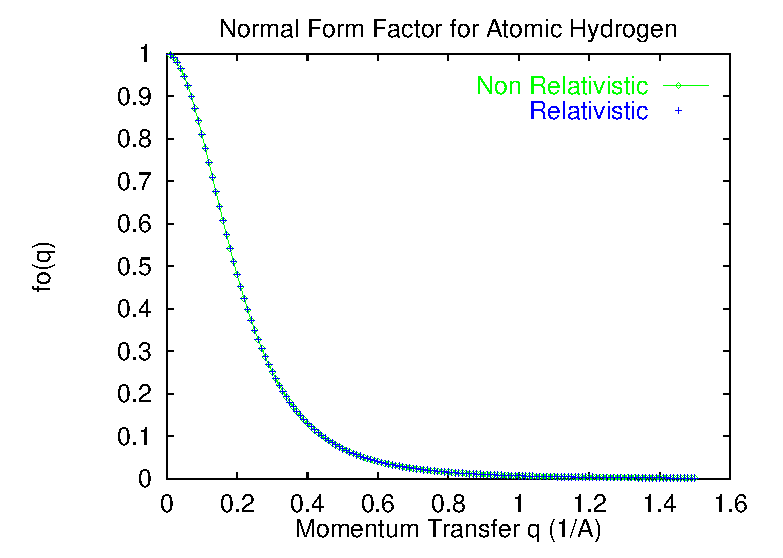
\includegraphics[width=7.0cm]{f0_hydrogen.eps}
        &
        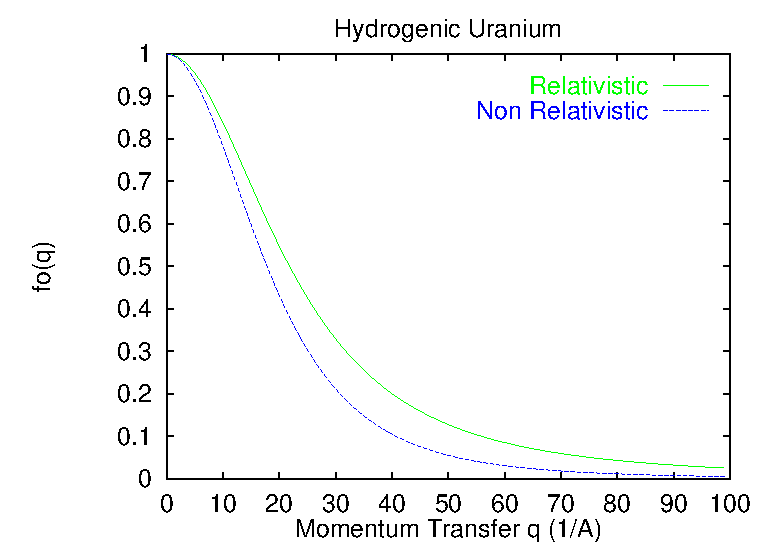
\includegraphics[width=7.0cm]{f0_uranium.eps}
    \end{tabular}
    \caption{Normal Form Factor for Single Electron Hydrogen and Uranium}
    \label{fig:hydrogen-uranium}
    \end{center}
    \end{figure}
    The relativistic normal form factor in equation~\ref{eq:nff-relativistic}
    can be compared to the non relativistic case by considering the small values
    of $Z$ in which the parameter $\gamma_1 = \sqrt{1-\alpha^2Z^2} \approx 1$. 
    In this case equation~\ref{eq:nff-relativistic} becomes:
    \begin{equation} \label{eq:reduction}
        f_0(q) \approx 
        2 \frac{\Gamma(2)}{\Gamma(3)}
        \left( \frac{2Z}{a_0} \right)^4
        \left[ 
            \left( \frac{2Z}{a_0} \right)^2 + q^2
        \right]^{-2} 
        =
        \left( \frac{2Z}{a_0} \right)^4
        \left[ 
            \left( \frac{2Z}{a_0} \right)^2 + q^2
        \right]^{-2} 
    \end{equation}
    which is in agreement with equation~\ref{eq:nff-nonrelativistic}.
    In figure~\ref{fig:hydrogen-uranium} we see plots for $f_0(q)$ comparing the non relativistic
    and relativistic results for standard atomic hydrogen and hydrogenic
    uranium.
    We can see that in the case of atomic hydrogen ($Z=1$), there is
    excellent agreement between the two results.
    In the case of hydrogenic uranium ($Z=92$) we can see that there is a
    significant difference over a range of momentum transfers between the
    relativistic and non relativistic results. 
    This shows the need for using relativistic Dirac wave functions as opposed to
    the Schr\"odinger wave functions when computing atomic form factors
    especially for heavier atoms.
    In figure~\ref{fig:hydrogen-uranium} it is difficult to make out difference
    between relativistic and non relativistic values for atomic hydrogen, since
    there seems to be quite good agreement between the two. However, if we plot
    the difference between the two results as is done in
    figure~\ref{fig:delta-theory}, we can clear identify the regions of momentum
    transfer where the relativistic theory is better even though the difference
    is of the order of $10^{-6}$ or less. We can see that the maximum
    difference between the two theories is at approximately $q = 0.3 \InvAngstrom$ and
    and it gets smaller at higher values of $q$.
    \begin{figure}[h]
    \begin{center}
        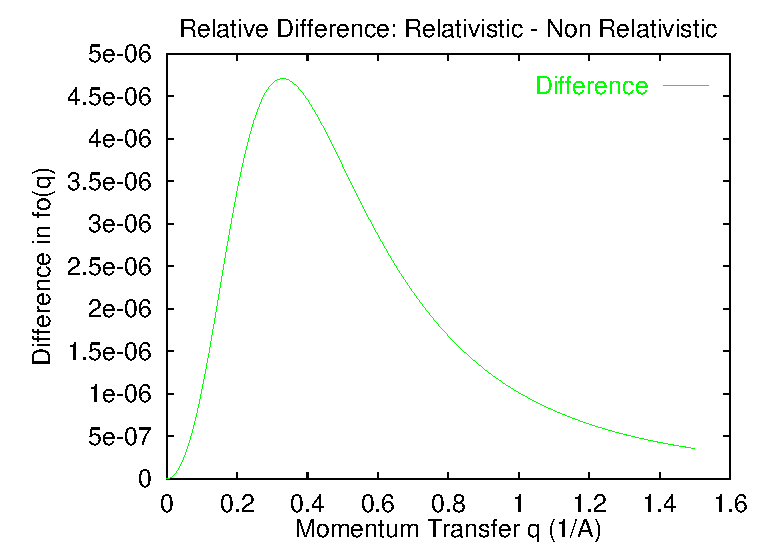
\includegraphics[width=7.0cm]{delta_theory.eps}
        \caption{Difference ($\Delta f_0(q)$) between relativistic and non relativistic theory}
        \label{fig:delta-theory}
    \end{center}
    \end{figure}

\section{Comparison with other theoretical results}
    \begin{figure}[H] 
    \begin{center}
    \begin{tabular}{cc}
        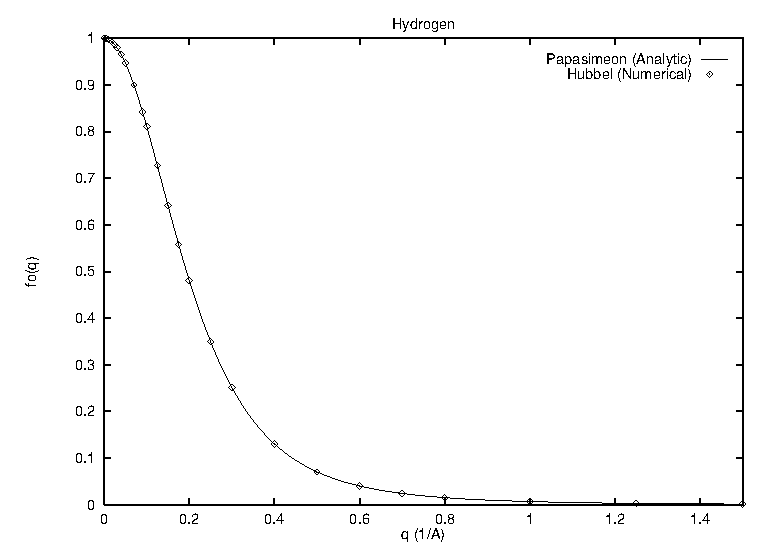
\includegraphics[width=7.0cm]{hubbel_papa.eps}
        &
        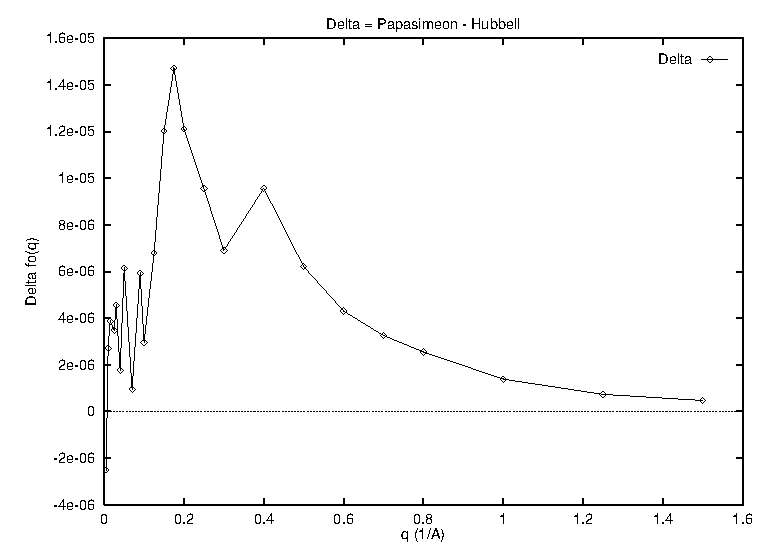
\includegraphics[width=7.0cm]{delta_hubbell.eps}
    \end{tabular}
        \caption{Normal Form Factor for Hydrogen -- Comparison With Hubbell's Theoretical Results}
        \label{fig:hubbell-comparison}
    \end{center}
    \end{figure}
    We can make a comparison between the results obtained using equation~\ref{eq:nff-relativistic}
    and other theoretical results which have used relativistic wave functions in
    computing $f_0(q)$.
    Tabulations of atomic form factors, incoherent scattering function and
    photon scattering cross sections were published by Hubbel et.  al.~\cite{Hubbell-1975}.
    The tabulations for the normal form factor for hydrogen used non
    relativistic wave functions. Figure~\ref{fig:hubbell-comparison} shows two
    plots comparing the analytic result of equation~\ref{eq:nff-relativistic} with
    Hubbel's tabulated results. The plot on the left shows good agreement, but
    looking at the difference between the two theories on the plot on the right
    shows the differences more clearly. The shape is similar to that shown
    in figure~\ref{fig:delta-theory} but the maximum difference is of the order
    of $10^{-5}$.


    % CHAPTER 4 - ANOMALOUS ATOMIC FORM FACTOR FOR HYDROGENIC ATOMS
    \chapter{ANOMALOUS FORM FACTOR FOR HYDROGENIC ATOMS}
        %%%%%%%%%%%%%%%%%%%%%%%%%%%%%%%%%%%%%%%%%%%%%%%%%%%%%%%%%%%%%%%%%%%%%%%%%%%%
%% PHOTOIONISATION
%%%%%%%%%%%%%%%%%%%%%%%%%%%%%%%%%%%%%%%%%%%%%%%%%%%%%%%%%%%%%%%%%%%%%%%%%%%%

\section{Computing $\mbox{\boldmath $f''(\omega)$ } $}
From equation~\ref{eq:fpp-sigma} we see that in order to determine the imaginary
component of the anomalous form factor $f''$ we need to know the total
photoionisation cross section. Therefore the basic tool that is required is the
computation of the photo-electric matrix element which will give as the
photoionisation amplitude. This matrix element can then be used in two
approaches to computing $f''$ such as:
\begin{itemize}
    \item Relativistic First Order Perturbation Theory
    \item Second Order S-Matrix Theory
\end{itemize}
We have concentrated on obtaining results for the form factor
using second order S-Matrix theory.
The purpose is to attempt to obtain analytic solutions to these problems.
Numerical techniques will be used when it is no longer possible to solve a
problem analytically.

\section{Amplitude for Photoionisation}
The relativistic photon absorption and emission operators for many electron atoms are 
defined~\cite{Kissel-S-Matrix} as:
\begin{eqnarray} \label{eq:photon-abs-emis}
    \mathcal{A}_i       & = & \sum_j \Alpha \cdot \hat{\epsilon}_j \Exp{k_i}{r_j} \\
    \mathcal{A}_f^{\dag}   & = & \sum_j \Alpha \cdot \hat{\epsilon}_j \ExpM{k_f}{r_j}
\end{eqnarray}
where the sum is over all the electrons in an atom, $\Alpha$ is the Dirac alpha
matrix, $\mb{r_j}$ is the position of the $j$-th electron, $\hat{\epsilon}_j$ is 
the polarisation of the photon and $\mb{k}$ is the wave vector of the photon.
The subscripts $i$ and $f$ indicate initial and final states respectively. This
is needed if we are considering for example Compton (inelastic) scattering where
the momentum of the photon changes in a scattering process. However, for the
case of Rayleigh scattering the photon momentum is unchanged 
($\hbar \omega_i = \hbar \omega_f$) and as such in this case we drop the
subscripts and just use the symbols $\omega$ and $\mb{k}$.
\begin{figure}[h]
    \begin{center}
        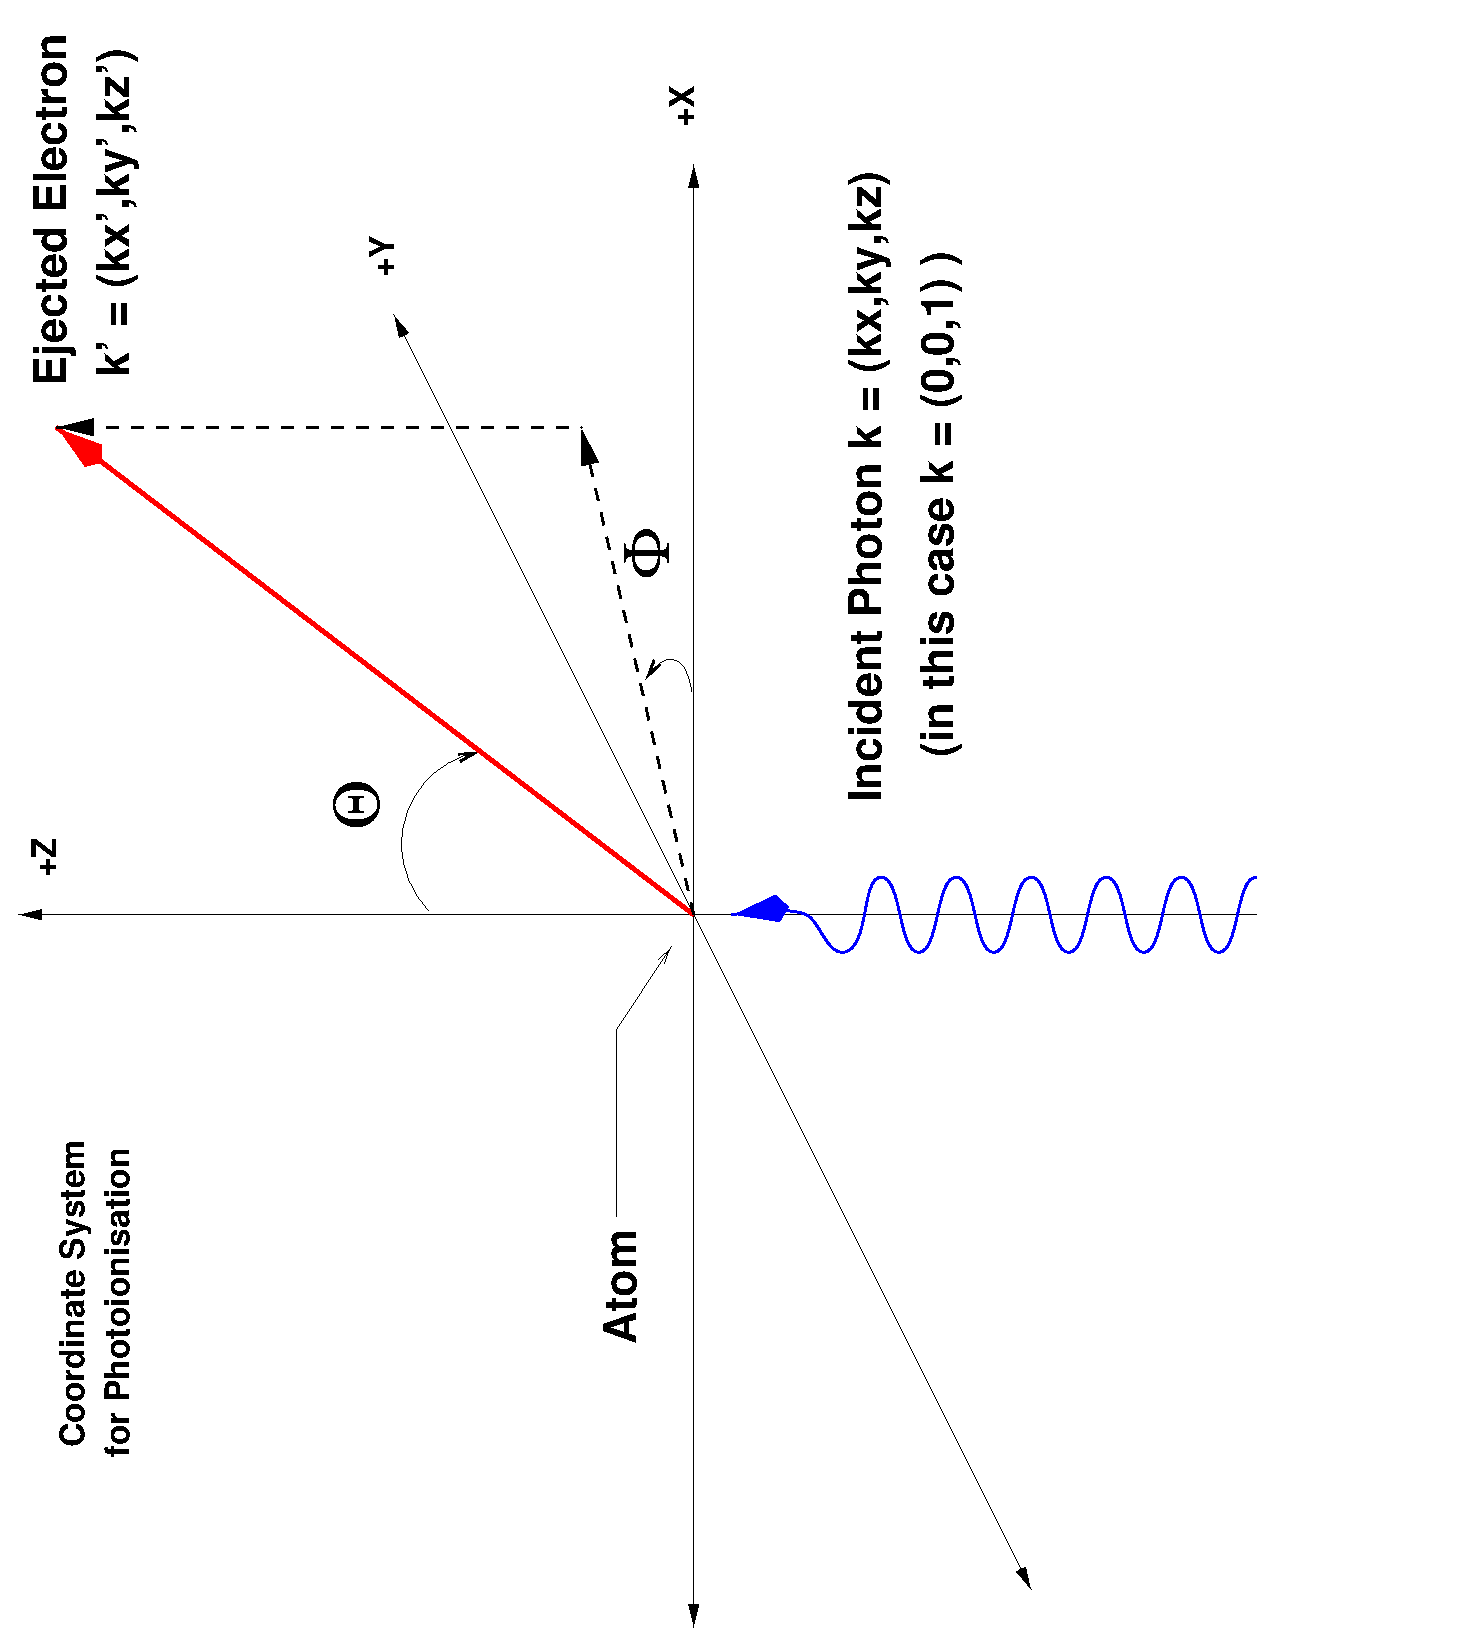
\includegraphics[angle=-90,width=7cm]{coords.eps}
    \end{center}
    \caption{Coordinate System for Photoionisation~\cite{Bransden-Joachain}}
    \label{fig:coordinates}
\end{figure}

We also need to define the coordinate system to be used to describe
photoionisation. The coordinate system setup is shown in figure~\ref{fig:coordinates}.
The small case angles $(\theta,\phi)$ are used to describe the
angular position of an electron bound to an atom, whereas the angles
$(\Theta,\Phi)$ are used to describe the electron ejected angle.
We make the following assumptions:
\begin{itemize}
    \item The incident photon has energy $\hbar \omega$ and is traveling
          in the $+Z$ direction with a momentum wave-vector 
          $\mb{k} = (k_x,k_y,k_z)$.
    \item The photon has a constant well defined polarisation. We will consider photon
          polarisations in the $x$ and $y$ directions. 
    \item The ejected electron has a wave-vector $\mb{k'} = {k'_x,k'_y,k'_y}$
          which defines its linear momentum and ejection direction/angles since:
          \begin{equation} \label{eq:ejection-angles}
          \begin{array}{cccc}
            k'_x & = & |k'| \sin(\Theta) \cos(\Phi) & \\
            k'_y & = & |k'| \sin(\Theta) \sin(\Phi) & \\
            k'_z & = & |k'| \cos(\Theta)&
          \end{array}
          \end{equation}
    \item The atom is initially in it's ground state, and is represented by a 
          $\ket{1S_{1/2}}$ (or $\ket{0}$ or $\psi_0$) wave-function 
          (non relativistic or relativistic).
    \item After photoionisation the ejected electron will be represented by a
          continuum (or free electron) state $\ket{c}$ (or $\psi_c$), 
          (non relativistic or relativistic).
\end{itemize}


\subsection{Photoionisation to a Continuum State}
    We first consider the first order photo-electric matrix element for a single
    electron atom using~\ref{eq:photon-abs-emis}:
    \(
        A_1 = \bra{\psi_c} \mathcal{A} \ket{\psi_0} = \bra{\psi_c} \Exp{k}{r} \Alpha_j \ket{\psi_0} .
    \)
    In the case that the incident photon is polarised either in the $x$ or $y$
    direction, and knowing that the second components of the ground state
    and continuum states are both zero ($\psi_{02} = 0$ and $\psi_{c2} = 0$)
    results in the following form for $A_1$:
    \[ 
        A_1 = \bra{\psi_c} \Exp{k}{r} \Alpha_j \ket{\psi_0} =
        \left\{ 
        \begin{array}{llllll} 

            \int \state{c}{1}^{*} \Exp{k}{r} \state{0}{4} \; d^3 \mb{r} 
            & + &
            \int \state{c}{4}^{*} \Exp{k}{r} \state{0}{1} \; d^3 \mb{r}
            & = & m_1 + m_2
            & \mbox{, if $j = x$} 

            \\[3mm]

            -i \int \state{c}{1}^{*} \Exp{k}{r} \state{0}{4} \; d^3 \mb{r}
            & + &
             i \int \state{c}{4}^{*} \Exp{k}{r} \state{0}{1} \; d^3 \mb{r}
            & = & -i m_1 + i m_2
            & \mbox{, if $j = y$} 

        \end{array} 
        \right .
    \]
    With known values for the spinor components $\state{c}{1}$, $\state{c}{4}$,
    $\state{0}{1}$ and $\state{0}{4}$ we can determine the integrals $m_1$ and
    $m_2$.

    With $\state{c}{1}^{*} = \ExpM{k'}{r}$ and 
    $\state{0}{4} = -i\sqrt{\frac{2}{3}} Y_{11}(\theta,\phi) f_0(r)
                  =  \frac{i}{\sqrt{4 \pi}} \sin(\theta) e^{i \phi} f_0(r)$
    we obtain for the $m_1$ integral:
    \[
    m_1 = \frac{i}{\sqrt{4\pi}} \int \sin(\theta) 
          e^{i \phi} \Exp{k}{r} \ExpM{k'}{r} f_0(r) \; d^3 \mb{r}
    \]
    To do the integration we change to spherical polar coordinates,
    $\mb{r} = r (\sin\phi \cos\theta,\sin\phi \sin\theta, \cos\phi)$, and we
    define 
    \begin{equation}
        \Muq = q_x \sin\phi \cos\theta + 
               q_y \sin\phi \sin\theta +
               q_z \cos\phi
    \end{equation}
    where $\mb{q} = \mb{k} - \mb{k'} = (q_x,q_y,q_z)$.
    Using the definition of $\Muq$ and using 
    $f_0(r) = F_0 G_0 r^{\gamma_1 - 1} e^{-\frac{1}{2}\sigma_1 r}$, $m_1$
becomes:
    \[
    m_1 = F_0 G_0 \frac{i}{\sqrt{4\pi}} \int
          \sin(\theta) e^{i\phi} e^{i\Muq} r^{\gamma_1 - 1} 
          e^{-\frac{1}{2}\sigma_1 r} \; d^3 \mb{r}
    \]
    We can now convert the integral over all space into one using spherical
    polar coordinates.
    \[
    m_1 = F_0 G_0 \frac{i}{\sqrt{4\pi}}
          \int_{0}^{2\pi}
          \int_{0}^{\pi}
          \int_{0}^{\infty}
            \sin^2(\theta) e^{i\phi} r^{\gamma_1 + 1}
            e^{-[ \frac{1}{2}\sigma_1 - i \Muq ] r }
          \; dr \; d\theta \; d\phi
    \]
    The angular integrations over $\theta$ and $\phi$ cannot be solved
    analytically due to the fact that $\Muq$ is a non simple function 
    of $\theta$ and $\phi$. However, using the fact that
    \(
        \int_0^\infty e^{-ax} dx = \Gamma(n+1)/a^{n+1}
    \)
    the radial integral can be solved.
    \[
    m_1 = \frac{i}{\sqrt{4\pi}} F_0 G_0 \Gamma(\gamma_1 + 2)
          \int_{0}^{2\pi}
          \int_{0}^{\pi}
            \left[
                \frac{\sin^2(\theta) e^{i\phi} }{
                    \left(
                        \frac{1}{2} \sigma_1 - i \Muq
                    \right)^{\gamma_1 + 2}
                }
            \right]
          \; d\theta
          \; d\phi
    \]

    We can determine the integral $m_2$ following a similar process to that used
    to determine $m_1$. In the case of $m_2$ the spinor components are given by
    $\state{c}{4}^{*} = \xi(k'_x - ik'_y)\ExpM{k'}{r}$ and 
    $\state{0}{1} = Y_{00}g_0(r) 
                  = \frac{1}{\sqrt{4\pi}} G_0
                     e^{-\frac{1}{2}\sigma_1 r} r^{\gamma_1 - 1}$
    we obtain for $m_2$:
    \[
    m_2 = \frac{\xi(k'_x -ik'_y)}{\sqrt{4\pi}} G_0 \Gamma(\gamma_1 + 2)
          \int_{0}^{2\pi}
          \int_{0}^{\pi}
            \left[
                \frac{\sin(\theta) }{
                    \left(
                        \frac{1}{2} \sigma_1 - i \Muq
                    \right)^{\gamma_1 + 2}
                }
            \right]
          \; d\theta
          \; d\phi
    \]
    
    Using $m_1$ and $m_2$ we can obtain an equation for the first order
    photo-electric amplitude $A_1(\mb{k},\mb{k'})_j$, where $j$ denotes 
    the polarisation direction.

        % X DIRECTION

    \begin{equation} \label{eq:A1-X}
    \boxed{
    A_1(\mb{k},\mb{k'})_x =
    \frac{G_0 \Gamma(\gamma_1 + 2)}{\sqrt{4\pi}}
    \int_{0}^{2\pi}
    \int_{0}^{\pi}
        \left[
            \frac {
            \sin(\theta) [ \xi(k'_x - ik'_y) + i F_0 \sin(\theta) e^{i\phi} ]
%                i F_0 \sin^2(\theta) e^{i\phi} + \xi(k'_x - ik'_y)\sin(\theta)
            } {
                (\frac{1}{2}\sigma_1 - i \Muq )^{\gamma_1 + 2}
            }
       \right]
    \; d\theta
    \; d\phi
    }
    \end{equation}

        % Y DIRECTION

    \begin{equation} \label{eq:A1-Y}
    \boxed{
    A_1(\mb{k},\mb{k'})_y =
    \frac{G_0 \Gamma(\gamma_1 + 2)}{\sqrt{4\pi}}
    \int_{0}^{2\pi}
    \int_{0}^{\pi}
        \left[
            \frac
            {
            i \sin(\theta) [ \xi(k'_x - ik'_y) - i F_0 \sin(\theta) e^{i\phi} ]
%                F_0 \sin^2(\theta) e^{i\phi} + \xi(k'_y + ik'_x)\sin(\theta)
            } {
                (\frac{1}{2}\sigma_1 - i \Muq )^{\gamma_1 + 2}
            }
        \right]
    \; d\theta
    \; d\phi 
    }
    \end{equation}
    These results have been derived without any approximations to the plane wave
    form of the electromagnetic field ($\Exp{k}{r}$) in the absorption and
    emission operators. This is the ``all poles'' approach. 
    In the electric dipole (E1) approximation we have $\Exp{k}{r} \approx 1$.
    We can interpret this as having no information about the propagation
    direction of the incident photon and hence in the electric dipole
    approximation $\mb{k} = 0$.
    Therefore to obtain results for the electric dipole approximation from
    equations~\ref{eq:A1-X} and~\ref{eq:A1-Y} it is simply a matter of
    setting $\mb{k} = 0$.
    \begin{equation} \label{eq:A1-Dipole}
    \boxed{
        A_1^{E1}(\mb{k},\mb{k'})_j = A_1(0,\mb{k'})_j
    }
    \end{equation}

\subsection{Photoionisation in the Forward Scattering Direction}
The integrals $m_1$ and $m_2$ defined in the previous section cannot be solved
analytically in general. However, it is possible to obtain an analytic solution 
for some special cases. One such case is when the incident photon is traveling
in the $+z$-direction with a propagation vector $k\hat{\mb{n}} = (0,0,k)$ and 
the electron is ejected in the $\Theta = 0$ (or forward scattering direction).
In this case, the propagation vector for the ejected electron is
$k'\hat{\mb{n}}' = (0,0,k')$.

We note from these assumptions that the integral $m_2 = 0$ because it is 
multiplied by the factor $\xi (k_x' - i k_y')$ and in the forward scattering
direction $k_x' = 0$ and $k_y' = 0$. We also note that the the function $\Muq$
is simplified to $\Muq = q_z \cos(\theta)$. We these new assumption we can 
rewrite the integral for $m_1$ and attempt an analytic solution.
\[
    m_1 = \frac{i}{\sqrt{4\pi}}
    \int_{0}^{\infty}
    \int_{0}^{2\pi}
    \int_{0}^{\pi}
        \sin^2(\theta) e^{iq_z \cos(\theta)} e^{i\phi} r^2 f_0(r) 
    \; d\theta
    \; d\phi
    \; dr
\]
Integrating over $\phi$ gives $2i$ and making use of the trigonometric
identity $2\sin^2(\theta) = 1-\cos(\theta)$, $m_1$ can be written as:
\begin{eqnarray*}
    m_1 & = & \frac{-2}{\sqrt{4\pi}}
    \int_0^\infty
        f_0(r) r^2
        \left[
            \frac{1}{2} 
            \int_0^\pi
                e^{i q_z r \cos(\theta) }
            \; d\theta
            +
            \frac{1}{2}
            \int_0^\pi
                \cos(2\theta) e^{i q_z r \cos(\theta) }
            \; d\theta
        \right]
    \; dr 
    \\
    & = &
    \frac{-2}{\sqrt{4\pi}}
    \int_0^\infty
    f_0(r) r^2
    \left[
        \frac{1}{2} ( \pi J_0(q_z r)  +  \pi J_2(q_z r) )
    \right]
    \; dr
    \\
    & = &
    \frac{-\pi F_0 G_0}{\sqrt{4\pi}}
    \left[
        \int_0^\infty
            J_0(q_z r) r^{\gamma_1 + 1} e^{-\frac{1}{2} \sigma_1 r}
        \; dr
        +
        \int_0^\infty
            J_2(q_z r) r^{\gamma_1 + 1} e^{-\frac{1}{2} \sigma_1 r}
        \; dr
    \right]
\end{eqnarray*}
where $J_n(x)$ is a Bessel function of the first kind of order $n$.
The integrals involving the Bessel functions can be solved in terms of the
hypergeometric function $_2 F_1(a,b;c;z)$~\footnote{These integrals were solved
using Mathematica 3.0}. Since $m_2$ is zero, the first order amplitude is given
in terms of $m_1$, where we have $A(k,k')_x = m_1$ and $A(k,k')_y = -i m_1$, for
photon polarisations in the $x$ and $y$ directions respectively. 
Using this information, and substituting in the for the constants $F_0$, 
$G_0$ and $\sigma_1$ which were defined earlier, the analytic solutions
for the first order photo-electric matrix elements in the forward scattering
direction are given by:
\begin{equation} \label{eq:A1-Forward}
\boxed{
\begin{split}
     A_1 & (k,k')_x  =  \frac{\pi}{\sqrt{\pi}}  
                        \left( \frac{2Z}{a_0} \right)^{3/2}
                        \sqrt{ \frac{1 - \epsilon_1}{
                                    2 \Gamma(2\gamma_1 + 1)
                               } } \times \\
    & \Biggl\{
        \left( \frac{Z}{a_0} \right)^{-(\gamma_1 + 2)}
    \Gamma(\gamma_1 + 2)
    \; _2 F_1 \left(
                \frac{\gamma_1 + 2}{2} ,
                \frac{\gamma_1 + 3}{2} ;
                1 ;
                - \left(
                    \frac{2a_0}{Z}
                \right)^2
                (k - k')^2
           \right)
    + \\ & 
    \frac{1}{8} (k - k')^2 
    \left( \frac{Z}{a_0} \right)^{-(\gamma_1 + 4)}
    \Gamma(\gamma_1 + 4)
    \; _2 F_1 \left(
                \frac{\gamma_1 + 4}{2} ,
                \frac{\gamma_1 + 5}{2} ; 
                1 ;
                - \left( \frac{2a_0}{Z} \right)^2
                (k - k')^2
            \right)
    \Biggr\}
\end{split}
}
\end{equation}
\begin{equation}
\boxed{
    A_1(k,k')_y = -i A_1(k,k')_x
}
\end{equation}
This implies that in the forward scattering direction, the probability of
photoionisation is the same for a photon polarised in the $x$ or $y$ direction,
because \( |A_1(k,k')_x|^2 = |A_1(k,k')_y|^2 \).

%%%%%%%%%%%%%%%%%%%%%%%%%%%%%%%%%%%%%%%%%%%%%%%%%%%%%%%%%%%%%%%%%%%%%%%%%%%%%%%%%%%%%%%%%
% S-MATRIX THEORY
%%%%%%%%%%%%%%%%%%%%%%%%%%%%%%%%%%%%%%%%%%%%%%%%%%%%%%%%%%%%%%%%%%%%%%%%%%%%%%%%%%%%%%%%%
\section{S-Matrix Theory}
S-matrix theory as developed in covariant perturbation theory (or quantum field
theory) is used to solve a large number of scattering problems in quantum
mechanics~\cite{Sakurai-Advanced,Greiner,Yndurain,Akhiezer,Weinberg}.
The use of S-matrix theory to compute atomic form factors has been applied by
Kissel and Pratt~\cite{Kissel-S-Matrix}.
For a given photon of energy $\hbar \omega$ the second order S-matrix (scattering) 
amplitude $A_2(\omega)$ is related to the imaginary component of the form factor 
$f''(\omega)$ and to the total cross section $\sigma^{TOT}(\omega)$ through the
following relation:
\begin{equation}
    \mathrm{Im} A_2(\omega) = r_0 f''(\omega) = \frac{\omega}{4 \pi c} \sigma^{TOT}(\omega)
\end{equation}
The relationship between the total cross section and $f''(\omega)$ is the same
as equation~\ref{eq:fpp-sigma}. Although here we will only be considering the
photoionisation cross section, $\sigma^{TOT}(\omega)$ may also include partial cross
section contributions from other process such as bound-bound transitions. 
In addition to this we also have that:
\begin{itemize}
    \item The second order amplitude considers only the forward scattering direction.\\
          $A_2(\omega) = A_2(\omega,\Theta=0)$.
    \item The sign of $f''$ as define by Kissel and Pratt~\cite{Kissel-S-Matrix} 
          is opposite of that used in the crystallography literature
          $(f''_{Kissel} = -f''_{cl})$. We will follow the convention of the
          crystallography community.
    literature.
\end{itemize}

The second order S-matrix amplitude is defined as follows:
\begin{equation}
     A_2 = 
     -r_0 mc^2 \sum_p
     \left[
     \frac{
        \bra{m} \mathcal{A}_f^\dag \ket{p}
        \bra{p} \mathcal{A}_i \ket{n}
     }{
        E_n - E_p + \hbar\omega_f + i0_+
     }
     +
     \frac{
        \bra{m} \mathcal{A}_i \ket{p}
        \bra{p} \mathcal{A}_f^\dag \ket{n}
     }{
        E_n - E_p - \hbar\omega_i + i0_+
     }
     \right]
\end{equation}
where the state $\ket{\psi}$ is a four component relativistic spinor which
satisfies the Dirac equation (equation~\ref{eq:dirac-equation}). The equation describes a second
order scattering process with the subscript $i$ denoting the initial situation
and $f$ denoting the final situation. The two components correspond to the
processes of photoabsorption followed by photoemission, and photoemission
followed by photoabsorption, as shown in the Feynmann diagrams in 
figure~\ref{fig:feynmann}.
\begin{figure}[h]
    \begin{center}
        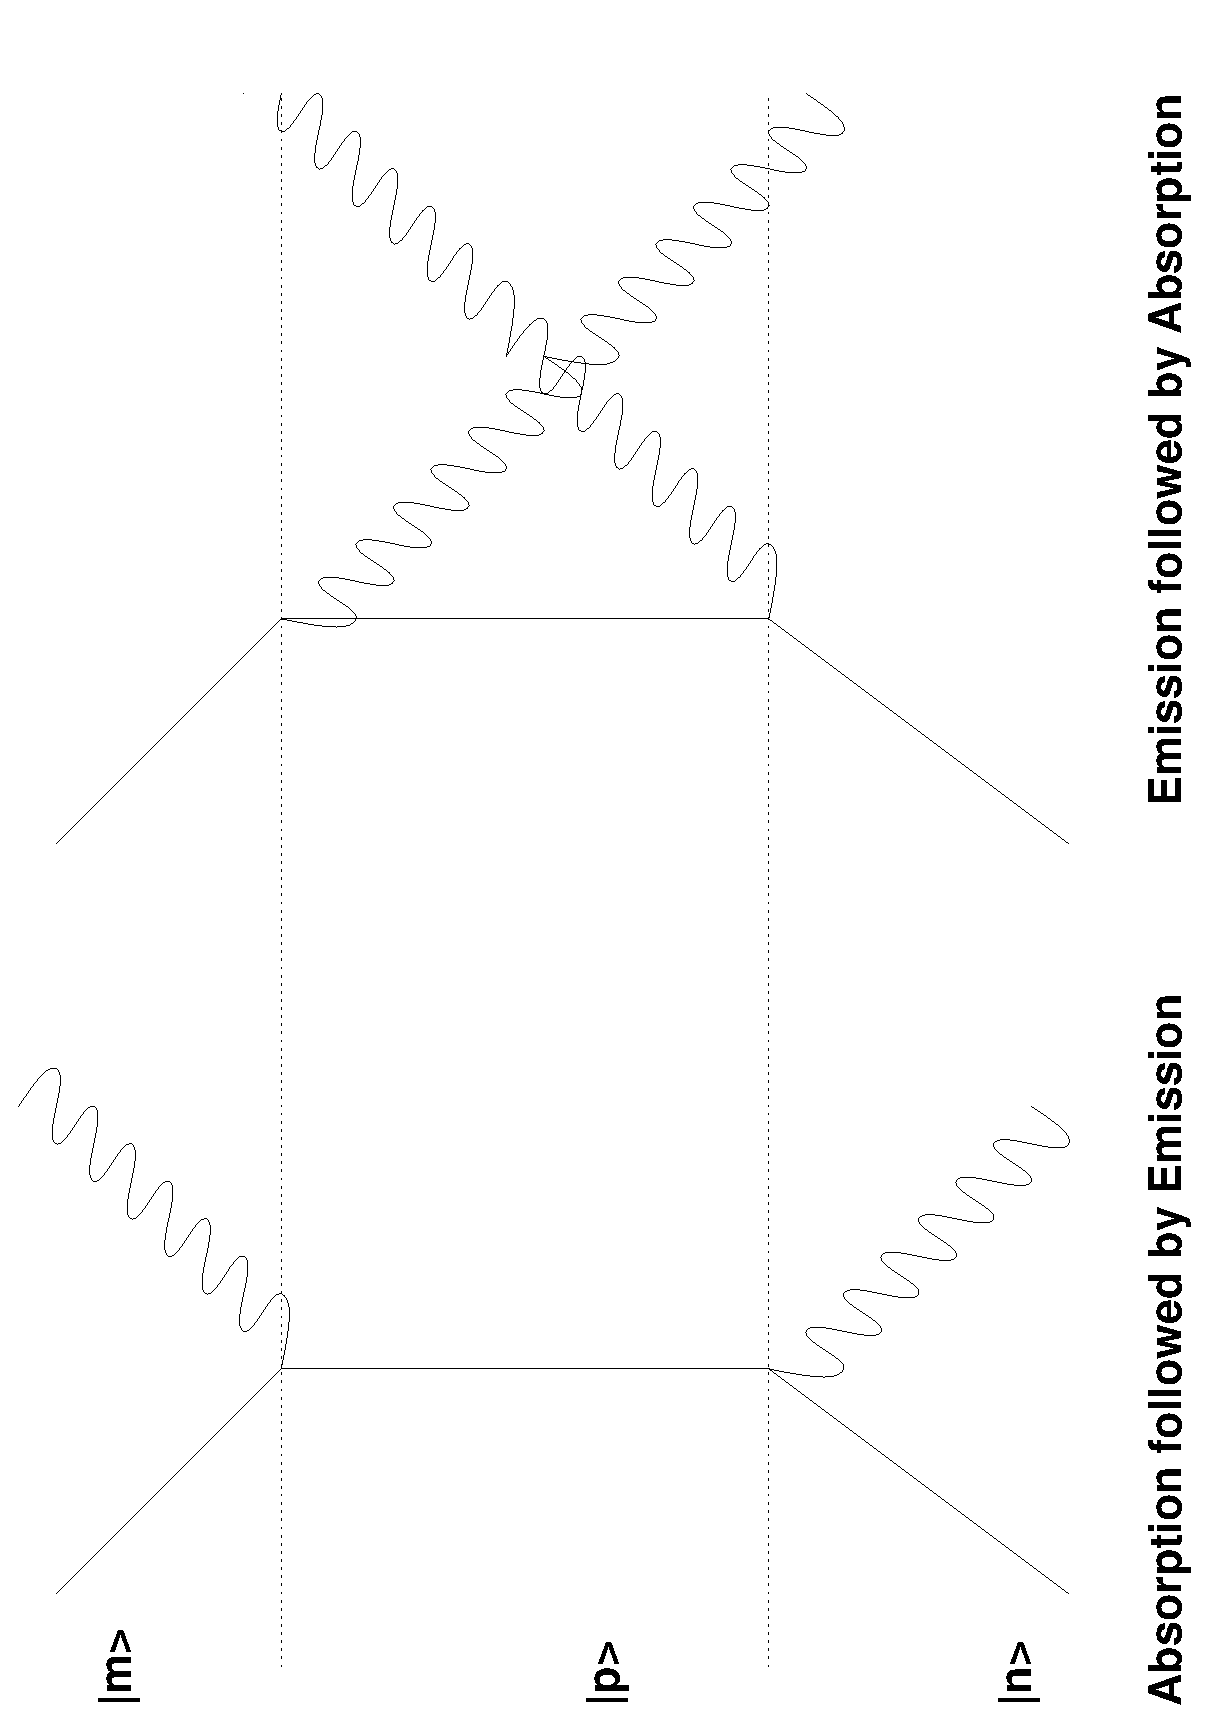
\includegraphics[angle=-90,width=7.0cm]{feynmann.eps}
    \end{center}
    \caption{Second Order Photon Scattering}
    \label{fig:feynmann}
\end{figure}

The initial state of the atom (which we will make
the ground state) is $\ket{n}$, the final state is $\ket{m}$ and we have
a sum of all intermediate states $\ket{p}$. The energy of the initial state is
$E_n$, the energy of the intermediate states is $E_p$, and initial and and final
energy of the photon are $\hbar \omega_i$ and $\hbar \omega_f$ respectively.
The denominator of both components of $A_2(\omega)$ includes a small complex
positive value $i0_+$.

For the case of Rayleigh scattering, 
$\hbar \omega_i = \hbar \omega_f = \hbar \omega$, and the final atomic state is the
same as the the initial atomic state ($\ket{n} = \ket{m}$). 
We can then define the form factor $f''$ in terms of the second order elastic
(Rayleigh) S-matrix $\mathrm{Im}A_2^R(\omega)$.
\begin{equation}
    f''(\omega) = \frac{\mathrm{Im}A_2^R(\omega)}{r_0} 
                = \frac{\omega}{4\pi c r_0} \sigma^{TOT}(\omega)
\end{equation}
If the initial state is the ground state of the hydrogen atom $\ket{\psi_0}$,
and we substitute in for the the emission and absorption operators previously
defined (without the summation since we only have a single electron) we 
obtain:
\begin{equation}
        A_2^R(\omega) = 
        -r_0 mc^2 \sum_p \left[
        \frac{
            \bra{\psi_0} \ExpM{k}{r} \Alpha_j \ket{\psi_p} 
            \bra{\psi_p} \Exp{k}{r}  \Alpha_j \ket{\psi_0}
        }{
            E_0 - E_p + \hbar\omega + i0_+
        } 
     +
        \frac{
           \bra{\psi_0} \Exp{k}{r}   \Alpha_j \ket{\psi_p} 
           \bra{\psi_p} \ExpM{k}{r}  \Alpha_j \ket{\psi_0} 
        }{
           E_0 - E_p - \hbar\omega - i0_+
        }
        \right]
\end{equation}
Making use of 
\(
    \bra{a} X^\dag \ket{b} \bra{b} X \ket{a} 
  = \bra{b} X \ket{a}^* \bra{b} X \ket{a} = | \bra{b} X \ket{a} |^2
\)
and splitting the sum into a sum over discrete states (bound excited states of
the hydrogen atom) and an integral over 
continuum states ($\ket{\psi_c}$ is the free electron continuum state) we obtain:
%\begin{equation}
%\begin{split}
\begin{multline}
    A_2^R(\omega)   =  
         -r_0 mc^2  \int_0^\infty
        \left[
             \frac{
            | \bra{\psi_c} \Exp{k}{r}  \Alpha_j \ket{\psi_0} |^2
        }{
            E_0 - E_c + \hbar\omega + i0_+
        } 
        +
        \frac{
           | \bra{\psi_c} \ExpM{k}{r}  \Alpha_j \ket{\psi_0} |^2
        }{
           E_0 - E_c - \hbar\omega - i0_+
        }
        \right]
        dEc
        \\
         -r_0 mc^2  \sum_p 
        \left[
        \frac{
            | \bra{\psi_p} \Exp{k}{r}  \Alpha_j \ket{\psi_0} |^2
        }{
            E_0 - E_p + \hbar\omega + i0_+
        } 
     +
        \frac{
           | \bra{\psi_p} \ExpM{k}{r}  \Alpha_j \ket{\psi_0} |^2
        }{
           E_0 - E_p - \hbar\omega - i0_+
        }
        \right]
\end{multline}
%\end{split}
%\end{equation}
Ideally both continuum and bound-bound components would be included in
a calculation of the S-matrix amplitude. However, due to time constraints the
calculations focused on the continuum component. From the standard
non relativistic understanding of the photo-electric 
effect~\cite{Sakurai-Modern,Kissel-S-Matrix,Chantler-Book} we know that the 
ground state to continuum amplitude dominates over the bound-bound transition
amplitudes. However Chapter 5 of this report contains some results for
bound-bound, transitions which may be used as a basis for determining 
atomic form factors.

Therefore, we can now write down the second order S-matrix amplitude which needs
be calculated. We see that the matrix elements in the numerators are simply
the first order photoionisation matrix elements 
(equations~\ref{eq:A1-X},~\ref{eq:A1-Y},~\ref{eq:A1-Forward}) so we can write
the second order amplitude in terms of first order amplitudes.
($\omega = kc$).
\begin{equation} \label{eq:A2}
\boxed{
     A_2^R(\omega) = A_2(\mb{k},\mb{k'})_j =
         -r_0 mc^2  
        \left[
        \int_0^\infty
             \frac{
             | A_1(\mb{k},\mb{k'})_j |^2
        }{
            E_0 - E_c + \hbar\omega + i0_+
        } 
        dEc
        +
        \int_0^\infty
        \frac{
            |A_1(\mb{-k},\mb{k'})_j |^2
        }{
           E_0 - E_c - \hbar\omega - i0_+
        }
        dEc
        \right]
}
\end{equation}
The second order amplitude for the electric dipole approximation, 
as for the first order matrix elements is simply given by setting $\mb{k}=0$.
\begin{equation} \label{eq:A2-Dipole}
    \boxed{
       A_2^{E1}(\mb{k},\mb{k'})_j  = A_2(0,\mb{k'})_j  
    }
\end{equation}
\subsection{Computational Method}
To compute $f''$, we need to compute the value of equation~\ref{eq:A2} 
over a range of photon energies ($\hbar \omega$), 
take the imaginary component and then divide by $r_0$.
This was done by developing a computer program in the C++ language to perform 
the computations using
numerical integration methods to solve the integrals in equations~\ref{eq:A1-X}
and~\ref{eq:A1-Y} and the integral over the continuum state (ejected electron
energies).
\begin{itemize}
    \item One of the main computation issues faced was the problem of multi 
          dimensional integrals. Although there was a single outer integral
          over continuum energies to compute the first order matrix element
          required the numerical computation of a two dimensional angular integral.
    \item The integration methods used originally elementary algorithms 
          based on the Simpson's and Trapezoidal rules. The main problem with
          these methods was computation speed and accuracy.
          Performance and accuracy of results improved when the integration
          routines where changed to a 10-point Gauss-Legendre 
          integration method~\cite{Koonin}.
    \item The integration method used for the integral over continuum states
          had to handle integrating over a singularity. This was handled by
          implementing a numerical version of the Cauchy principal value
          technique~\cite{Engineering-Maths}. The integral was split into 
          three regions, below the singularity, near the singularity and
          above the singularity to infinity. The integral to infinity was
          numerically by making an appropriate change of variable, changing
          the integral from one that was over an open interval to one that
          was over a closed interval.
    \item All the computations where done in atomic units (a.u.) 
          giving the standard units of electrons/atom for $f''$.
          The energy axes in keV were converted after the computation
          was performed.
    \item Since $f''(\omega)$ is calculated using the imaginary component
          of the second order S-matrix amplitude the size of the small
          positive complex value $i0_+$ was expected to effect the results.
The pseudo-code below gives an outline of the depth level of all the
numerical integrations involved in the calculation, showing why computation
speed was an issue.
\end{itemize}
 \begin{verbatim} 
    PROGRAM
    {
        For E = Min_Photon_Energy To Max_Photon_Energy With Step=EnergyStep
            Compute 2nd Order Matrix Element
                Integrate A2 Over All Continuum Energies 
                    Compute 1st Order Matrix Element
                        Integrate Over Phi From 0 To 2Pi 
                            Integrate Over Theta From 0 To Pi
    } 
\end{verbatim}


\subsection{Results for $f''(\omega)$ and
            Possible Problems With S-Matrix Theory as Currently Implemented}
Figure~\ref{fig:compare-poles} shows a logplot the form factor ($\log_{10}(f'')$)
for a range of photon energies to 100 keV. The plot compares the result obtained
using the all poles approach with that obtained for $f''$ using the electric
dipole approximation. As can be seen, the all pole and electric dipole approach
are closer in agreement at lower energies. We expect that the electric dipole
approximation breaks down the higher the photon energy we have and this is
indeed the case in the results obtained. This is because the electric dipole
approximation makes the assumption that the wavelength of the photon is much
larger than the size of the atom it is interacting with. At higher energies,
and hence shorter wavelengths, this approximation begins to break down as
is evident in figure~\ref{fig:compare-poles}.
\begin{figure}[h]
\begin{center}
    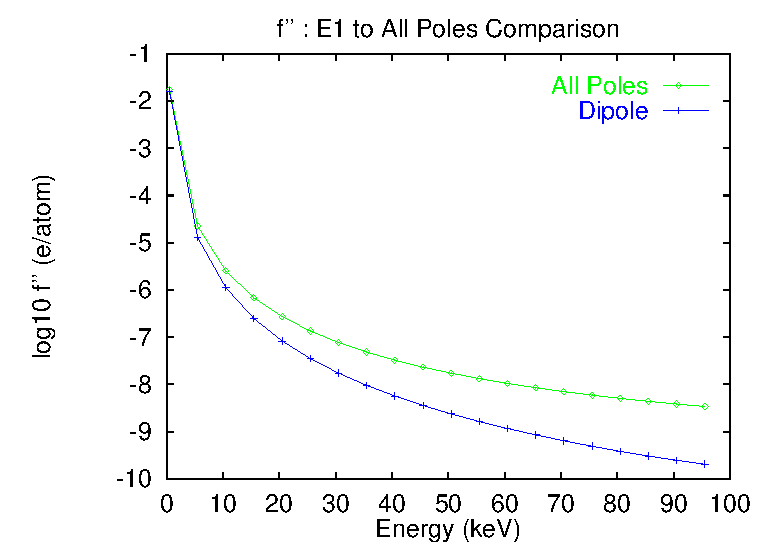
\includegraphics[width=7cm]{compare_poles_1.eps}
\end{center}
    \caption{Relativistic Form Factor $f''$ -- Comparing Electric Dipole 
            to All Poles Result}
    \label{fig:compare-poles}
\end{figure}
\begin{figure}[h]
\begin{center}
    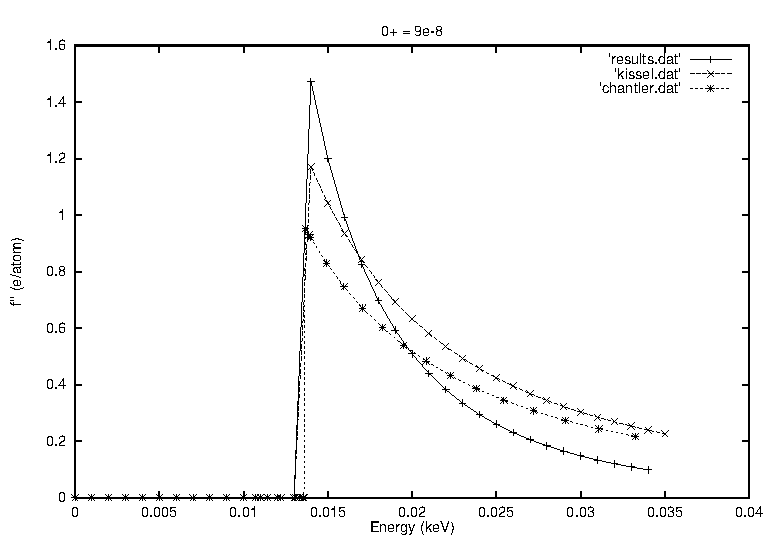
\includegraphics[width=7cm]{compare_fpp_1.eps}
    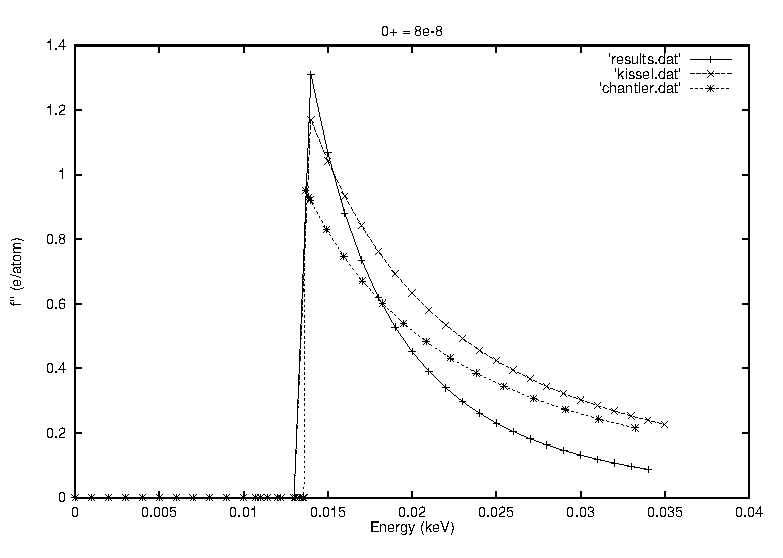
\includegraphics[width=7cm]{compare_fpp_2.eps}
    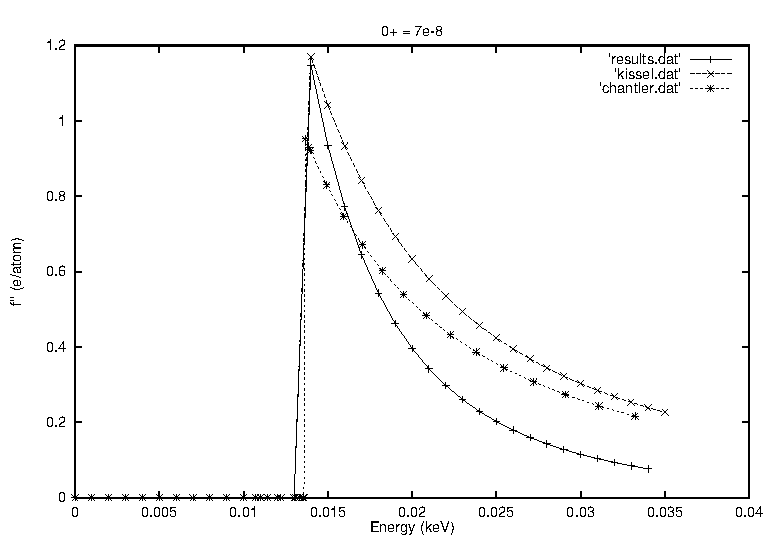
\includegraphics[width=7cm]{compare_fpp_3.eps}
    \caption{Comparing Current Results for $f''$ with those of Chantler
             and those of Kissel and Pratt}
    \label{fig:fpp-compare}
\end{center} 
\end{figure}
Figure~\ref{fig:fpp-compare} shows three plots of $f''(\omega)$ at an energy
range encompassing an edge (in this case the ionisation energy of the hydrogen
atom $E_0 = 13.6$ eV. The plots contain comparisons between these new results,
the S-matrix results of Kissel and Pratt~\cite{Kissel-S-Matrix}, and
the recent results of Chantler~\cite{Chantler-Tabulation}. 
The three plots show the new results for three different values of the
small complex value $i0_+ = 7\times 10^{-8},8\times 10^{-8},9\times 10^{-8}$.
Clearly, the results are affected by the change in size of $i0_+$.
All three theories predict the correct edge at 13.6 eV, all qualitatively
have a similar shape, but there is disagreement between all three.

With regards to the new results, there clearly are some issues that need
to be addressed. The main one is the dependence on $i0_+$. One way to attempt
to solve this problem would be to try to change the integration scheme used 
from a non-convergent method (Gauss-Legendre) used to obtain the current results
to a method such as a form of Romberg integration which converges to a result.
This may or may not fix the problem with regard to the size of $i0_+$.
If the problem still persists, then it could possibly suggest there are still
some problems with S-matrix theory as currently implemented in the area of
calculating atomic form factors.

\subsection{Results for Angular Dependence}
The mod-squared of the second order S-matrix element $|A_2(\mb{k},\mb{k'})_j|$
cannot also be used to study the angular distribution of the ejected electron
(or photoelectrons) at selected energies. We keep the direction
of the photon wave-vector the same ($\mb{k} = k(0,0,1)$) as when calculating
$f''$, just changing the magnitude for different photon energies. 
However the ejected electron wave vector is described by the ejection
angles $(\Theta,\Phi)$ (see equation ~\ref{eq:ejection-angles}). 
In the $f''$ case we were interested in the forward scattering direction
so we set $\Theta = 0$. Alternatively, we can set $\Phi = 0$ and vary
$\Theta$ over a range from $0$ to $2 \pi$. 
This gives as an ejected electron angular distribution for all values of $\Theta$ in
the $\Phi = 0$ plane.

\begin{figure}[h]
\begin{center}
\begin{tabular}{cc}
    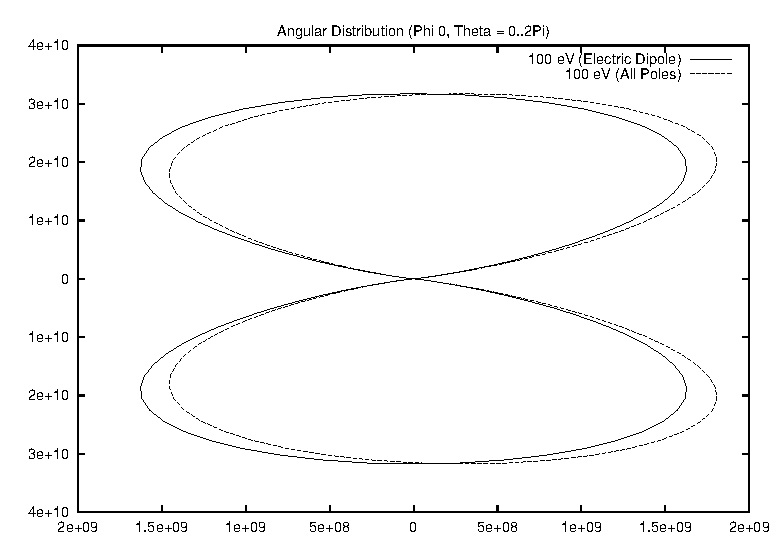
\includegraphics[width=7cm]{ang_100eV_both.eps}
    &
    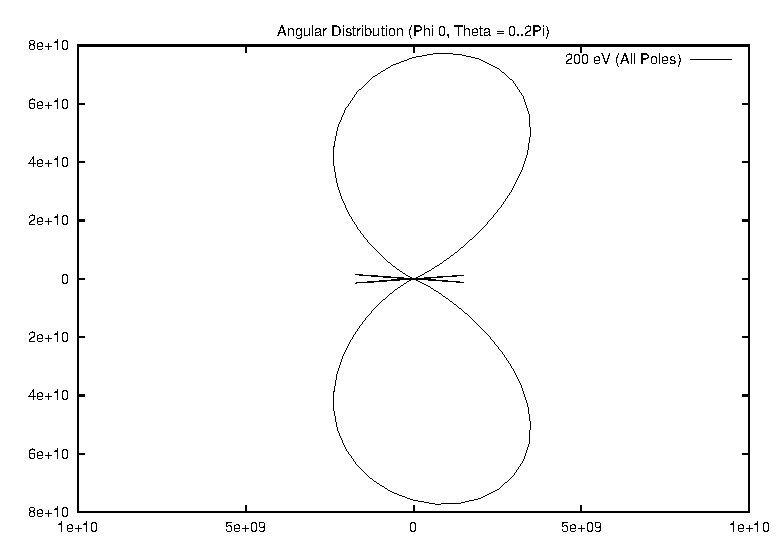
\includegraphics[width=7cm]{ang_200eV_ap.eps}
    \\
    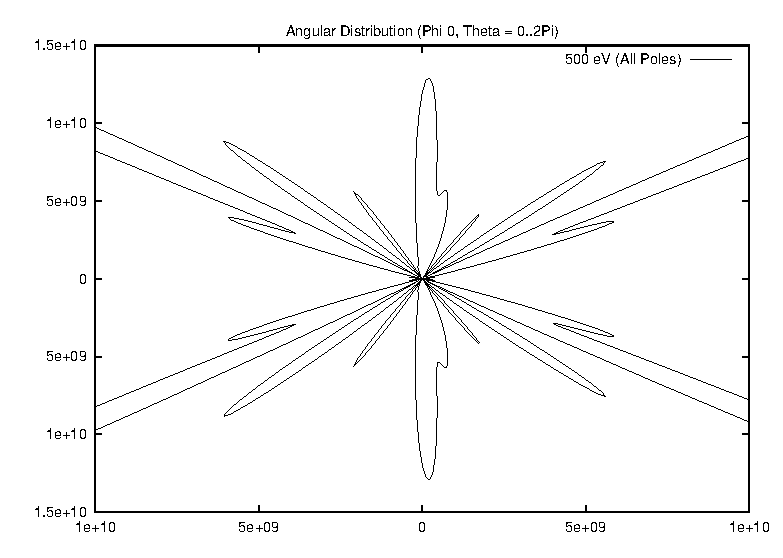
\includegraphics[width=7cm]{ang_500eV_ap.eps}
    &
    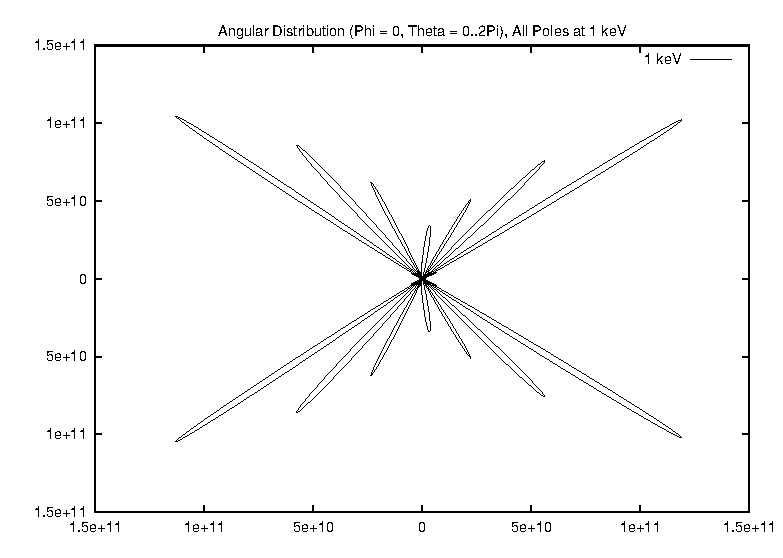
\includegraphics[width=7cm]{ang_1keV_ap.eps}
\end{tabular}
    \caption{Ejected Electron Angular Distributions at Photon Energies of
             100 eV, 200 eV, 500 eV and 1 keV}
    \label{fig:angular-plots}
\end{center}
\end{figure}

The results for $|A_2(\mb{k},\mb{k'})_j|$ at photon energies of
100 eV, 200 eV, 500 eV and 1 keV are shown in figure~\ref{fig:angular-plots}.
The top left plot for a photon energy of 100 eV also shows the distribution
for the electric dipole approximation. 
At the lower energies we see that the plots exhibit a $\sin^2(\Theta)$
distribution. As the energy is increased we see finer definition
of the ejection lobes in all directions, indicating the very precise
directions of electron ejection.


%%%%%%%%%%%%%%%%%%%%%%%%%%%%%%%%%%%%%%%%%%%%%%%%%%%%%%%%%%%%%%%%%%%%%%%%%%%%%%%%%%%%%%%%%
% RELATIVISTIC PERTURBATION THEORY
%%%%%%%%%%%%%%%%%%%%%%%%%%%%%%%%%%%%%%%%%%%%%%%%%%%%%%%%%%%%%%%%%%%%%%%%%%%%%%%%%%%%%%%%%
%\section{Relativistic Perturbation Theory}
%\begin{equation}
%    \frac{d\sigma}{d\Omega} =
%    \frac{\alpha k'}{2 m_e \pi \omega}
%    | \bra{\psi_c} \Exp{k}{r} \Alpha \cdot \hat{\epsilon}_j \ket{\psi_0} |^2
%    = \frac{\alpha k'}{2 m_e \pi \omega} |A_1(k,k')_j|^2 
%\end{equation}



    % CHAPTER 5 - BOUND-BOUND TRANSITIONS
    \chapter{ATOMIC BOUND-BOUND TRANSITIONS}
        
\section{Ground State to an Excited Bound State}
We mentioned in Chapter 5 that ideally the total cross section would have both
amplitudes corresponding to ground-continuum transitions and bound-bound
transitions. The first step that is required is to calculate a photoabsorption
matrix element from the ground state to one of the excited bound
states of hydrogen. 

This chapter provides semi analytic results for photoabsorption matrix elements
from the ground state to the first three excited states of hydrogen.
We will consider the the relativistic absorption operator $\mathcal{A} = \Alpha_x \Exp{k}{r}
= \Alpha_x e^{i\eta(\mb{k},\theta,\phi)r}$ for a photon polarised in the $x$
direction and we define $\eta$ as:
\begin{equation}
    \eta(\mb{k},\theta,\phi) = k_x \sin\phi \cos\phi +
                               k_y \sin\phi \sin\theta +
                               k_z \cos\phi
\end{equation}
In the electric dipole approximation $\mb{k} = 0$ and hence $\eta = 0$. 
The use of $\eta$ allows us to separate the angular and radial integrals
therefore writing the photoabsorption matrix element from the ground
state $\ket{\psi_0}$ to an excited bound state $\ket{\psi_i}$ as:
\begin{equation}
    \bra{\psi_i} X \ket{\psi_0}
    =
    \int (A_{i1}A_{01} + A_{ii}A_{0i}) R^g_{0i} \; d\Omega
    +
    \int (A_{i3}A_{03} + A_{i4}A_{04}) R^h_{0i} \; d\Omega
\end{equation}
where $A_{ij}(\theta,\phi)$ are the angular components of the excited 
state Dirac spinors as defined in Chapter 2.
$R^g_{0i}$ and $R^h_{0i}$ are the large and small component radial 
integrals which are defined in the sections below for each excited state.
Some of the radial integrals are analytic while others have to be solved
numerically. The final integration over all angles $ d\Omega $ has to 
be performed numerically.

All the radial integrals are written in terms of the constants defined in
Chapter 2 and in terms of the integrals $\mathcal{J}$ and $\mathcal{K}$ 
defined below.
\begin{equation}
    \mathcal{J}[a,n] = \int_0^\infty e^{-ar} r^n \; dr
\end{equation}
\begin{equation}
    \mathcal{K}[a,n,A,B,C,D] = \int_0^\infty 
                \left( \frac{A-Br}{C-Dr} \right) e^{-ar} r^{n} \; dr
\end{equation}

\section{Ground State to First Excited State}
\begin{equation}
R^g_{01} = G_0 G'_1 \mathcal{J}[\Half(\sigma_1 + \sigma_2) - i\eta,2\gamma_1] -
           G_0 G''_1 \mathcal{J}[\Half(\sigma_1 + \sigma_2) - i\eta,2\gamma_1 + 1]
\end{equation}

\begin{equation}
\begin{split}
R^h_{01} = H_0 G_0 H_1 
            G'_1 \mathcal{K}[\Half(\sigma_1 + \sigma_2) - i\eta, 2\gamma_1,H'_1,H''_1,H'''_1,H''''_1]
            \\ -
   H_0 G_0 H_1          G''_1 \mathcal{K}[\Half(\sigma_1 + \sigma_2) - i\eta, 2\gamma_1,  1H'_1,H''_1,H'''_1,H''''_1]
\end{split}
\end{equation}

\section{Ground State to Second Excited State}
\begin{equation}
R^g_{02} = G_0 G'_2 \mathcal{J}[\Half(\sigma_1 + \sigma_2) - i\eta,2\gamma_1] -
           G_0 G''_2 \mathcal{J}[\Half(\sigma_1 + \sigma_2) - i\eta,2\gamma_1 + 1]
\end{equation}

\begin{equation}
\begin{split}
R^h_{02} = H_0 G_0 H_2 
            G'_1 \mathcal{K}[\Half(\sigma_1 + \sigma_2) - i\eta, 2\gamma_1,H'_2,H''_2,H'''_2,H''''_2]
            \\ - 
   H_0 G_0 H_2          G''_1 \mathcal{K}[\Half(\sigma_1 + \sigma_2) - i\eta, 2\gamma_1, 1H'_2,H''_2,H'''_2,H''''_2]
\end{split}
\end{equation}

\section{Ground State to Third Excited State}
\begin{equation}
R^g_{03} = G_0 G_3 \mathcal{J}[\Half(\sigma_1 + \sigma_3) - i\eta, \gamma_1 + \gamma_2]
\end{equation}

\begin{equation}
R^h_{03} = H_0 G_0 H_3 G_3 \mathcal{J}[\Half(\sigma_1 + \sigma_3) - i\eta, \gamma_1 + \gamma_2]
\end{equation}



    % CHAPTER 5 - SUMMARY OF NEW RESULTS
    \chapter{SUMMARY OF NEW RESULTS}
        \section{New Results}

\begin{itemize}
\item We show a new result for the relativistic normal form factor
      for hydrogenic atoms in equation~\ref{eq:nff-relativistic}.
\item We show that for low Z atoms (non-relativistic limit)
      the relativistic normal form factor reduces to the non
      relativistic normal form factor for hydrogen in equation~\ref{eq:reduction}.
\item We compare and look at the differences between the new relativistic
      form factor and the non relativistic theory~\ref{eq:nff-nonrelativistic}
      and an alternate theory (Hubbell) and graphically
      show the differences in figures~\ref{fig:delta-theory} 
      and~\ref{fig:hubbell-comparison}

\item We show semi-analytic results for the first order relativistic
photoabsorption amplitude for photons polarised in both the $x$ and $y$
directions for the all poles approach (equations~\ref{eq:A1-X}
and~\ref{eq:A1-Y}) 
and for the electric dipole approximation (equation~\ref{eq:A1-Dipole}).

\item We show a new complete analytic result for the first order
photoabsorption amplitude in the forward scattering direction
(equation~\ref{eq:A1-Forward}).

\item We show a result for the second order S-matrix amplitude for the
      all poles (equation~\ref{eq:A2}) and electric dipole 
      approximation (equation ~\ref{eq:A2-Dipole}).

\item We present a result in figure~\ref{fig:compare-poles} for the normal form factor $f''$
      in both the all poles approach and the electric dipole approximation
      over a range of energies.

\item We compare the results obtained for $f''$ near an absorption edge for
      hydrogen with other theories (see figure~\ref{fig:fpp-compare}).

\item We show results for angular the angular distribution of ejected 
      photoelectrons at selected energies (see figure~\ref{fig:angular-plots}).

\end{itemize}

\section{Further Work In This Area}
    The work presented in this thesis can be expanded in a number of different
    ways. Firstly, the integration techniques used in the S-matrix theory can
    be improved to hopefully provide more accurate results.
    Secondly, the first order photoionisation amplitudes can be used
    to calculate a first order photo-electric cross section which 
    can then be used to calculate $f''$, which may then be compared
    to the results obtained with the second order S-matrix theory.
    Thirdly, the cross section components due to bound-bound transitions,
    and other effect such as Delbr\"uck and Compton scattering and pair
    production should be added to the existing photoionisation 
    cross section.

    Longer term research in the area of relativistic atomic form factors
    can include calculations for molecular hydrogen, bound hydrogen, and a study
    of the multiple scattering processes which give rise to XAFS (X-Ray
    Anomalous Fine Structure).
    Additionally, the development form factor calculations for many electron
    atoms ranging from Helium to Uranium making use of numerical 
    relativistic Dirac-Hartree-Fock wave-functions is also of great interest.




    % BIBLIOGRAPHY
    \bibliographystyle{acm}
    \bibliography{references}

\end{document}
